%% =====================================================================
%% FYDP-III FINAL REPORT (complete)  —  Group B1, UIU CSE
%% Self-Healing SDN using Reinforcement Learning
%%
%% This is the COMPLETE report: it keeps all content from the original
%% FYDP__III_Group_B1_252.pdf, completes the sections that were only
%% headings (Chapter 5 Standards & Design Constraints), and integrates
%% the actual experiments built after the small testbed (fault
%% localization at scale, real OFPFlowMod recovery, best-path resolver,
%% online day-by-day learning, and a full end-to-end run).
%%
%% Build on Overleaf / TeX Live:
%%   pdflatex fydp_report_full -> pdflatex (x2 for TOC/refs)
%% Uses only standard, Overleaf-bundled packages.
%% Numbers marked % [VERIFIED ...] trace to files under docs/ + results/.
%% =====================================================================
\documentclass[12pt,a4paper]{report}
\usepackage[margin=1in]{geometry}
\usepackage{graphicx}
\usepackage{booktabs}
\usepackage{amsmath}
\usepackage{array}
\usepackage{tikz}
\usetikzlibrary{positioning}
\usepackage{pgfplots}
\pgfplotsset{compat=1.16}
\usepackage{algorithm}
\usepackage{algpseudocode}
\usepackage{caption}
\usepackage[hidelinks]{hyperref}

\title{\textbf{Self-Healing SDN using Reinforcement Learning:\\
An Approach to Autonomous Fault Recovery}}
\author{}
\date{}

\begin{document}

% ---------- Title page ----------
\begin{titlepage}
\centering
\vspace*{2cm}
{\LARGE\bfseries Self-Healing SDN using Reinforcement Learning:\\[6pt]
An Approach to Autonomous Fault Recovery\par}
\vspace{2cm}
{\large By\par}
\vspace{0.5cm}
\begin{tabular}{ll}
Argha Biswas & 011221293\\
Ashikur Rahaman & 001221292\\
Md.\ Mizanur Rahaman & 011221381\\
Md Tarik Hasan & 011221585\\
Akram Hossain & 011221446\\
Apu Halder & 011221517\\
\end{tabular}
\vspace{1.5cm}

{\large Submitted in partial fulfilment of the requirements\\
of the degree of Bachelor of Science in Computer Science and Engineering\par}
\vspace{1cm}
{\large February 28, 2026\par}
\vspace{1.5cm}
{\large Supervised by\\ Dr.\ Al-Sakib Khan Pathan\\ Professor, Department of Computer
Science and Engineering\par}
\vspace{1cm}
{\large Department of Computer Science and Engineering\\
United International University\par}
\end{titlepage}

% ---------- Abstract ----------
\chapter*{Abstract}
\addcontentsline{toc}{chapter}{Abstract}
Software-Defined Networking (SDN) centralises control and makes network management
programmable, which improves operational efficiency but also concentrates the risk of
link and path failures in the control plane. Conventional fault handling still relies on
static backup paths or manual reconfiguration that react slowly to failures. This project
presents a self-healing SDN controller that closes the full recovery loop: it continuously
reads OpenFlow telemetry, detects and localises a fault, selects the best surviving path,
and installs the corresponding flow rules (\texttt{OFPFlowMod}) to reroute traffic, then
learns from the outcome so that its choices improve over time. The system is implemented on
Mininet with the Ryu controller and Open vSwitch, and every stage is evaluated under
leakage-free protocols rather than a single favourable run. Fault detection reaches
$0.94$ held-out accuracy; a hybrid of OpenFlow port-status and telemetry localises every
injected hard fault ($19/19$) across two topologies with no congestion false alarms; a
loss-aware path selector beats loss-blind recovery in three of five live scenarios and
matches a ground-truth oracle; event-driven recovery completes within about $40$~ms; and,
on a drifting network where the decisive signal is not observable at decision time, an
online reinforcement-learning rule keeps recovery quality high while a frozen model
collapses ($p=0.0039$ over eight seeds). A single live run composes all stages and adapts
its path preference as the network changes. A recurring, honest finding is that the value
lies in the integrated closed loop and in learning where it matters (the sequential
recovery policy), rather than in a learned detector, for which a lightweight classifier
suffices. All controllers, topologies, the fault-injection harness, and evaluation scripts
are released for reproducibility.

% ---------- Acknowledgements ----------
\chapter*{Acknowledgements}
\addcontentsline{toc}{chapter}{Acknowledgements}
This work would not have been possible without the input and support of many people over
the last two trimesters. We express our gratitude to everyone who contributed to it in some
way. First, we sincerely thank our academic supervisor, Dr.\ Al-Sakib Khan Pathan, for his
guidance, patience, and continuous encouragement throughout the project. We are grateful to
the faculty and staff of the Department of Computer Science and Engineering at United
International University for providing the resources and environment that made this work
possible. Last but not least, we owe a debt of gratitude to our families, including our
parents, for their unconditional love and immense emotional support.

% ---------- Publication list ----------
\chapter*{Publication List}
\addcontentsline{toc}{chapter}{Publication List}
The main contributions of this research are being prepared for submission to a
peer-reviewed venue.
\begin{description}
\item[Journal / Conference Papers (in preparation):] ``Self-Healing SDN using
Reinforcement Learning: An Approach to Autonomous Fault Recovery,'' Group B1, Department of
CSE, United International University.
\end{description}

\tableofcontents
\listoffigures
\listoftables

% =====================================================================
\chapter{Introduction}
The introduction chapter provides an overview of the project and explains its motivation,
objectives, methodology, outcomes, and the organisation of the report.

\section{Project Overview}
\begin{figure}[t]
\centering
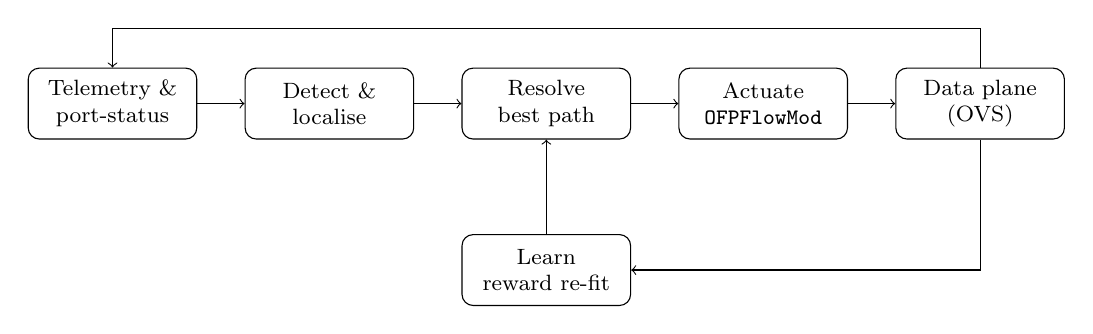
\begin{tikzpicture}[font=\footnotesize,
  box/.style={draw, rounded corners, align=center, minimum height=9mm,
              text width=20mm, inner sep=2pt}]
\node[box] (tel) {Telemetry \&\\port-status};
\node[box, right=6mm of tel] (det) {Detect \&\\localise};
\node[box, right=6mm of det] (res) {Resolve\\best path};
\node[box, right=6mm of res] (act) {Actuate\\\texttt{OFPFlowMod}};
\node[box, below=12mm of res] (learn) {Learn\\reward re-fit};
\node[box, right=6mm of act] (net) {Data plane\\(OVS)};
\draw[->] (tel) -- (det); \draw[->] (det) -- (res); \draw[->] (res) -- (act);
\draw[->] (act) -- (net);
\draw[->] (net.north) -- ++(0,5mm) -| (tel.north);
\draw[->] (net.south) |- (learn.east);
\draw[->] (learn.north) -- (res.south);
\end{tikzpicture}
\caption{System design: the closed-loop self-healing pipeline. The controller reads
telemetry and port-status, detects and localises a fault, resolves the best recovery path,
installs it with \texttt{OFPFlowMod}, and learns from the measured outcome.}
\label{fig:system-design}
\end{figure}

The system design in Figure~\ref{fig:system-design} highlights the connection between the
data plane, the decision logic, and the SDN controller. The design enables autonomous and
adaptive responses to link failures and congestion, supporting efficient fault detection,
proactive management, and improved network reliability and service continuity.

Software-Defined Networking (SDN) operates through two main parts: the control plane and
the data plane. In this project we use that separation to build a system that manages
faults and congestion automatically. The data plane forwards packets and exposes real-time
statistics such as throughput, packet loss, and delay. The controller processes these
metrics to identify signs of failure or congestion, decides how to recover, and then applies
the change to the data plane, for example by rerouting traffic onto a healthy path to bring
the network back to acceptable performance.

\subsection*{Problem Statement}
Static backups and manual reconfiguration are common in SDN fault handling, but they are
often too slow and too rigid for large, changing networks. This project addresses how an SDN
can automatically and efficiently detect and recover from different faults (such as link
failures, node failures, and congestion), while reducing downtime and packet loss.

\section{Motivation}
Modern networks such as cloud, IoT, and 5G demand high availability and rapid response to
faults. Manual troubleshooting and static recovery strategies do not scale to the size and
variability of current networks. A learning-based controller can (i) learn good recovery
decisions from interaction with the network, (ii) adapt to conditions that were not seen at
design time, and (iii) improve long-term performance by minimising packet loss and recovery
latency. A self-healing SDN can reduce operational cost, improve service robustness, and
strengthen resilience for mission-critical applications.

\section{Objectives}
The objectives of this project are:
\begin{enumerate}
\item Design a controller that works with an SDN control plane to automatically detect,
localise, and repair network faults.
\item Build a working prototype on an SDN testbed (Mininet with the Ryu controller and Open
vSwitch).
\item Inject a range of network problems (single- and multi-link failure, node failure, and
congestion) and recover from them by rerouting and updating flow tables.
\item Evaluate the system against baseline methods using detection time, recovery time,
packet loss, throughput, and path quality.
\item Assess how the system behaves as the network grows and as failure conditions change
over time.
\end{enumerate}

\section{Methodology}
A concise summary of the methodology:
\begin{itemize}
\item \textbf{Literature review:} survey SDN fault management and learning-based control.
\item \textbf{Testbed setup:} build an emulated SDN with Mininet, Open vSwitch, and Ryu.
\item \textbf{Fault injection:} inject single-link, multi-link, node, and congestion faults
for training and testing.
\item \textbf{Decision and recovery design:} detect and localise faults, generate candidate
recovery paths, score them with a multi-objective utility, and actuate the chosen path.
\item \textbf{Learning:} record the outcome of each recovery as a reward and re-fit the
decision policy from recent experience.
\item \textbf{Evaluation:} compare against static and load-aware baselines and a
ground-truth oracle using the metrics above, over multiple seeds.
\end{itemize}

\section{Project Outcome}
\begin{itemize}
\item A working closed-loop self-healing SDN controller that not only decides but also
actuates recovery through \texttt{OFPFlowMod}.
\item Quantitative, verified results showing accurate localisation, fast recovery,
loss-aware path selection, and day-by-day improvement, compared against honest baselines.
\item Guidance on safe operation (fail-secure installation, validation-guarded learning
updates) and a released, reproducible artifact (controllers, topologies, fault harness, and
evaluation scripts).
\end{itemize}

\section{Organization of the Report}
The rest of the report is organised as follows. Chapter~2 reviews recent work on SDN fault
tolerance and learning-based networking (2020--2025) and identifies the gaps that motivate
this work. Chapter~3 presents the system design: the architecture, the testbed, fault and
traffic generation, and the detailed methodology, including the detection, resolution, and
learning components. Chapter~4 covers implementation, engineering challenges, and the
experimental results, from single-fault recovery to localisation at scale, best-path
resolution, online learning, and a full end-to-end run. Chapter~5 discusses standards and
design constraints, cost, and the project timeline. Chapter~6 concludes with a summary and
limitations.

% =====================================================================
\chapter{Background}
This chapter reviews the fundamental concepts and prior work, identifies the research gaps,
and motivates the proposed approach.

\section{Preliminaries}
Software-Defined Networks (SDNs) separate the control plane from the data plane, allowing
centralised control and flexible programmability of network behaviour. This architecture
improves efficiency for managing traffic, recovering from faults, and automating network
behaviour compared with traditional static networks. Centralised control lets an SDN
dynamically configure itself and adapt to changing conditions, which is the property this
project exploits for autonomous recovery.

\section{Literature Review}
Recent studies apply machine learning (ML), deep learning (DL), and reinforcement learning
(RL) to improve the performance and reliability of SDNs. Some address congestion control,
while others focus on detecting and recovering from faults.

Boussaoud \emph{et al.} (2025) studied intelligent congestion detection and traffic control
in SDNs using data-driven multi-agent RL agents on Mininet and Ryu, reporting precision
above $0.91$ and recall of $0.94$--$0.97$. Huang \emph{et al.} (2025) proposed a
DDPG-based link-backup-path method for fast faulty-link recovery in SDN-based wide-area
monitoring, reducing recovery time by about $12\%$ and loss by about $15\%$ on IEEE test
topologies. Kumar \emph{et al.} (2023) reviewed AI-driven methods for self-healing networks,
describing how Q-learning and deep learning support fault detection and recovery, and
recommending hybrid RL models. Neto \emph{et al.} (2020) built a self-healing SDN/NFV
control-plane platform based on RL and topology encoding for link-failure recovery. Hammad
\emph{et al.} (2023) improved SDN intrusion recovery with ML and RL, reporting large
recovery-time reductions. Jo \emph{et al.} (2024) applied deep RL to self-healing in radial
distribution networks. Li \emph{et al.} (2022) designed an RL life-cycle framework (RLOps)
for Open RAN. Younisse \emph{et al.} (2024) reviewed multi-agent RL for self-healing and
fault isolation with 5G and fog computing. Sahu \emph{et al.} (2023, 2019) developed
RL-based methods for cyber-resilient power systems and simultaneous service restoration and
load management.

\subsection{Similar Applications}
Several web and mobile tools apply SDN and AI principles to network management and
monitoring, including traffic-optimisation tools, fault-detection dashboards, and controller
interfaces that automate configuration and recovery. They share goals with the proposed
system but typically use different methodologies and integrate learning differently.

\subsection{Related Research}
Table~\ref{tab:related} summarises representative learning-based SDN and self-healing work
and positions this project against it. Despite rapid progress, several challenges remain
with existing solutions:
\begin{itemize}
\item Congestion-control algorithms are often heuristic and static, performing poorly under
dynamic traffic and complex topologies.
\item Large-scale fault-recovery methods typically do not consider multi-fault or cascading
failures.
\item Existing methods usually address congestion control \emph{or} fault recovery
separately, without an integrated solution.
\item Online adaptation and continual learning are largely unexplored, limiting real-time
self-healing.
\item Practical deployment aspects, including scale and edge constraints, are seldom
addressed.
\end{itemize}
This project addresses these gaps with an integrated, adaptive self-healing SDN framework
that combines fault localisation, loss-aware recovery, real actuation, and online learning.

\begin{table}[t]
\centering
\footnotesize
\caption{Comparison of representative learning-based methods for congestion control and
fault recovery in SDNs.}
\label{tab:related}
\begin{tabular}{@{}p{2.3cm}p{3.2cm}p{3.0cm}p{3.4cm}@{}}
\toprule
\textbf{Work} & \textbf{Problem} & \textbf{Method / Tools} & \textbf{Key results} \\
\midrule
Boussaoud (2025) & Congestion detection and control & Mininet/Ryu, multi-agent RL (DQN) &
Precision $\ge0.91$, recall $0.94$--$0.97$ \\
Huang (2025) & Faulty-link recovery (WAMS) & DDPG, IEEE 30/57 topologies & Delay $\downarrow$
$12\%$, loss $\downarrow$ $15\%$ \\
Kumar (2023) & Survey of self-healing networks & Q-learning, deep learning & Lower false
positives, higher adaptability \\
Neto (2020) & Control/mgmt-plane self-healing & RL, topology encoding & Higher resilience,
efficient rerouting \\
Hammad (2023) & Intrusion recovery & ML (SVM/RF) + RL & Recovery time reduced substantially \\
Li (2022) & RL life-cycle for Open RAN & RLOps, digital twin, Kubernetes & Secure, scalable
RL deployment \\
\textbf{This work} & Integrated SDN self-healing & Detect $\rightarrow$ localise
$\rightarrow$ resolve $\rightarrow$ learn on Mininet/OVS/Ryu & Closed loop with real
actuation; honest baselines (oracle, widest-path, adaptive) \\
\bottomrule
\end{tabular}
\end{table}

\section{Summary}
This chapter introduced SDN concepts and learning-based techniques for network optimisation,
reviewed related research on congestion control and fault recovery, and identified the gaps:
the need for an integrated, adaptive, and scalable solution that both decides and actuates
recovery and that keeps improving as the network changes.

% =====================================================================
\chapter{Project Design}
\section{Methodology and Implementation}

\subsection{Context Diagram}
The context diagram represents the interaction between the system components and external
entities such as network operators and the SDN data plane. The operator configures policies
and observes status; the controller observes the data plane through OpenFlow and acts on it
by installing flow rules.
\begin{figure}[t]
\centering
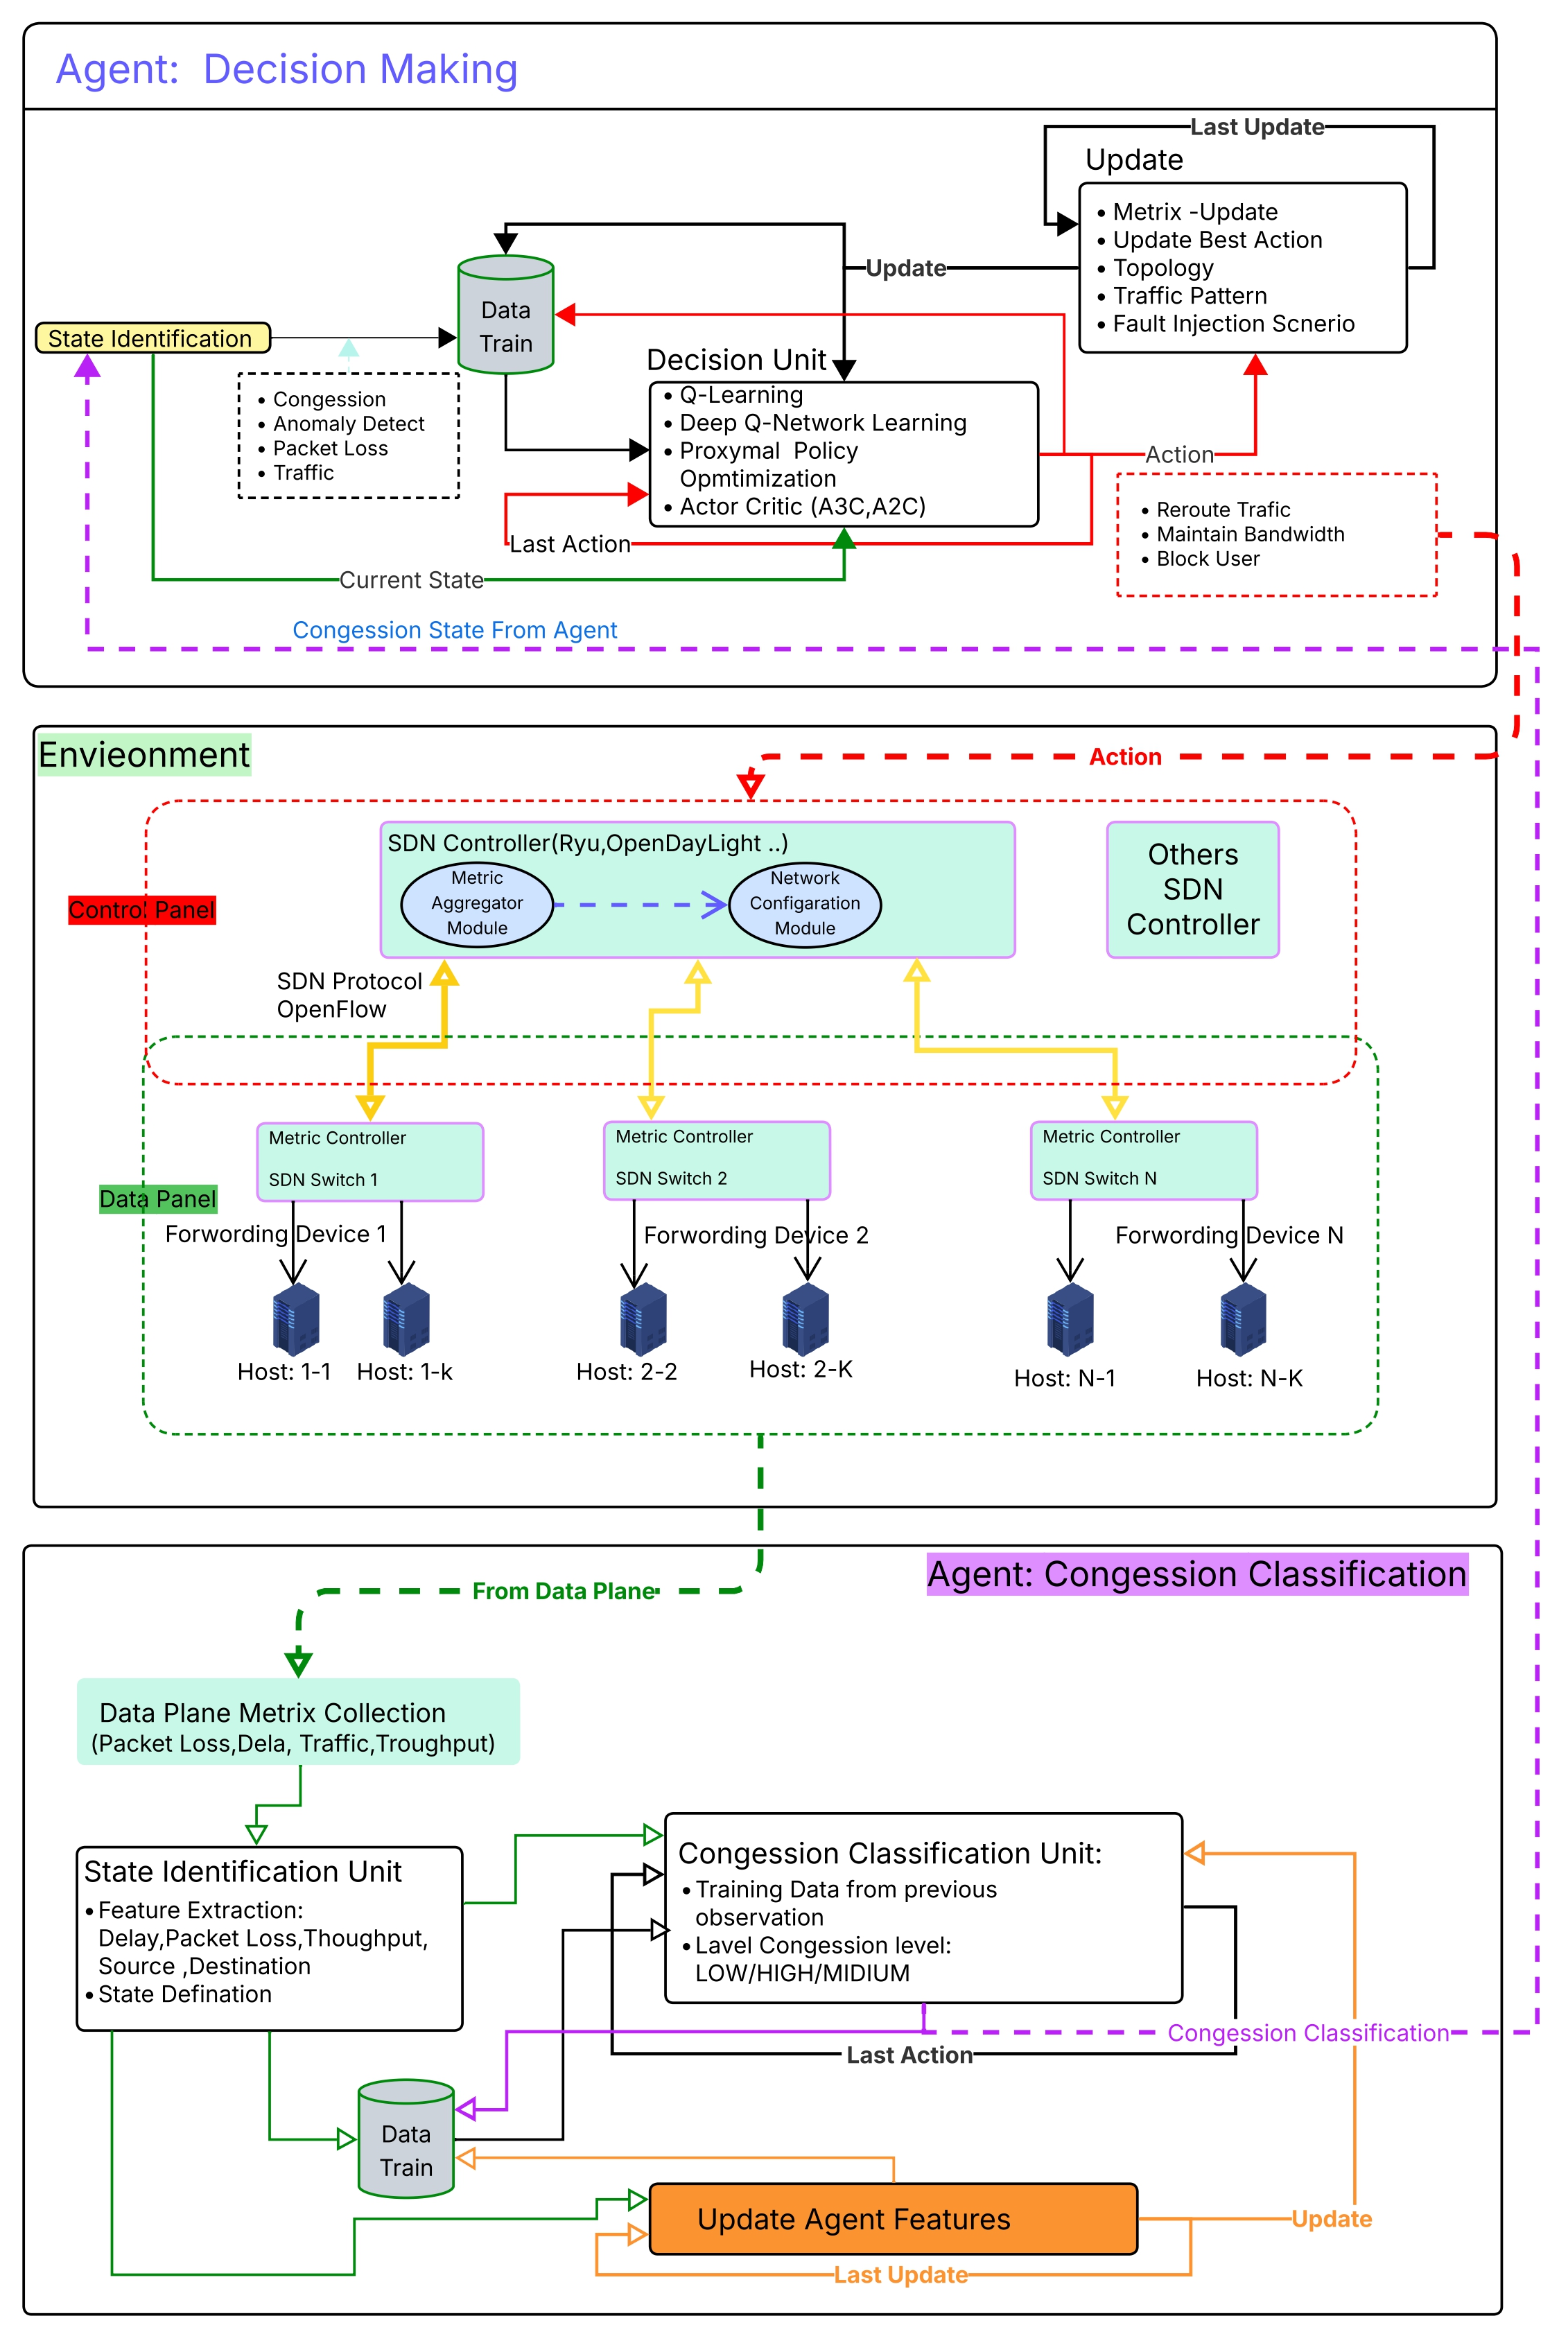
\includegraphics[height=0.82\textheight,keepaspectratio]{figures/context_diagram.png}
\caption{Context diagram of the proposed system: the state-identification and congestion
classification agent, the SDN environment (control and data planes), and the decision-making
agent that acts on the network.}
\label{fig:context}
\end{figure}

\subsection{System Architecture}
The proposed self-healing SDN framework is organised as a set of cooperating components that
separate the extraction of network state from the decision and recovery process
(Figure~\ref{fig:system-design}).
\begin{itemize}
\item \textbf{State-identification unit:} running on top of the Ryu OpenFlow controller,
this unit continuously polls the data plane to extract raw port statistics and compute
normalised telemetry (throughput, loss, delay). It also consumes OpenFlow port-status events
for exact fault localisation.
\item \textbf{Decision unit:} this unit detects whether a fault has occurred and, on a
fault, selects the best surviving path. Detection can use a Proximal Policy Optimization
(PPO) model or a lightweight classifier; path selection uses a multi-objective resolver.
\item \textbf{Actuation unit:} the controller translates the chosen path into per-switch
\texttt{OFPFlowMod} rules and installs them fail-secure.
\item \textbf{Learning unit:} each recovery's measured outcome is turned into a reward and
used to re-fit the resolver's weights from recent experience, so the policy adapts over time.
\end{itemize}

\subsection{Testbed Environment}
A virtualised testbed emulates an enterprise network. The data plane is emulated with
Mininet using Open vSwitch (OVS) and OpenFlow~1.3; the control plane is the Ryu controller in
a Python virtual environment on an Ubuntu Linux machine. Two topologies are used. For the
initial detection study, a small linear topology with a redundant backup link prevents
broadcast storms while allowing multi-hop rerouting. For the framework experiments, a
seven-switch mesh provides three node-disjoint paths between the endpoints with distinct
bandwidth and delay: Path~A (5~Mb/s, 2~ms), Path~B (10~Mb/s, 5~ms), and Path~C (20~Mb/s,
10~ms). A second mesh topology is used to test that fault localisation generalises.

\subsection{Data Generation and Fault Injection}
A custom Python harness drives Mininet through distinct phases to produce a diverse dataset
and to exercise recovery:
\begin{enumerate}
\item \textbf{Low congestion:} baseline reachability with ICMP ping.
\item \textbf{Medium-to-high congestion:} heavy UDP flows with \texttt{iperf} to overwhelm
switch buffers and induce loss and latency.
\item \textbf{Fault injection:} administrative disabling of links (single and multiple),
node isolation, and controlled congestion, to simulate hardware and cable failures as well
as gray failures.
\end{enumerate}

\subsection{Detailed Methodology and Design}
The self-healing mechanism follows a continuous closed-loop pipeline: network-state
monitoring, state normalisation, fault detection and localisation, best-path resolution,
autonomous actuation, and policy update from the observed outcome.

\subsubsection{State Identification and Normalisation}
The controller queries the OpenFlow switches every three seconds for
\texttt{OFPPortStatsReply} messages. The raw byte difference is converted to kilobits per
second and scaled to $[0,1]$ so that large-valued features (throughput) do not overshadow
smaller but important ones (loss) during learning. Algorithm~\ref{alg:telemetry} details the
extraction and normalisation.

\begin{algorithm}[t]
\caption{Real-time telemetry extraction and normalisation via Ryu}
\label{alg:telemetry}
\begin{algorithmic}[1]
\State Initialise \textit{port\_stats} and \textit{req\_times} dictionaries
\While{controller is active}
  \ForAll{connected datapaths (switches)}
    \State record current timestamp in \textit{req\_times}
    \State send \texttt{OFPPortStatsRequest} to the datapath
  \EndFor
  \State wait 3 seconds
\EndWhile
\Statex
\State \textbf{on receiving} \texttt{OFPPortStatsReply}:
\State $\textit{delay} \gets \text{now} - \textit{req\_times}[\textit{dpid}]$
\ForAll{ports in the datapath}
  \State $\textit{curr\_bytes} \gets \textit{rx\_bytes} + \textit{tx\_bytes}$
  \If{previous stats exist}
    \State $\textit{tput} \gets ((\textit{curr\_bytes}-\textit{prev\_bytes})\times 8)/
      (\textit{time\_diff}\times 1000)$
    \If{$\textit{tput} = 0$} \State $\textit{loss} \gets 1.0$ \Comment{zero-packet logic}
    \Else \State $\textit{loss} \gets (\textit{rx\_drops}+\textit{tx\_drops})/
      (\textit{curr\_pkts}-\textit{prev\_pkts})$ \EndIf
    \State $\textit{state} \gets [\min(\textit{tput}/25000,1),\ \min(\textit{loss},1),\
      \min(\textit{delay}/100,1)]$
    \State forward \textit{state} to the decision unit
  \EndIf
  \State update previous stats
\EndFor
\end{algorithmic}
\end{algorithm}

\subsubsection{Fault Localisation}
Detecting that a fault exists is not the same as knowing which link failed. A per-port
telemetry classifier cannot localise reliably, because a failed link and its innocent
downstream neighbours lose traffic in the same way. The framework therefore uses OpenFlow
port-status events for exact localisation (immune to congestion, since a congested link
stays up) and reserves telemetry for confirming service impact and for gray failures.

\subsubsection{Best-Path Resolution}
On a localised fault, the controller builds the current topology graph with the failed
element removed, enumerates candidate paths with a $k$-shortest-paths search (Yen's
algorithm), and scores each candidate $p$ with a scale-free multi-objective utility:
\begin{equation}
U(p) = w_1(-\ell_p) + w_2\, c_p + w_3(-L_p) + w_4(-h_p),
\label{eq:objective}
\end{equation}
where $\ell_p$ is latency, $c_p$ bottleneck capacity, $L_p$ loss, and $h_p$ hop count, each
min--max normalised across the candidate set. Recovery weights are fixed a priori at
$w=[0.5,1.0,1.5,0.1]$. % [VERIFIED docs/s2_5_results.txt]
The best path is compiled to per-switch \texttt{OFPFlowMod} rules.

\subsubsection{Decision and Learning}
For the binary detection decision (maintain or reroute), a PPO model is trained with an
oversampled, class-balanced dataset and a symmetric reward, as in
Algorithm~\ref{alg:ppo}. For adaptation, each completed recovery yields an outcome
(throughput, remaining loss, recovery time) that is scored by a reward
$r=\beta\cdot\text{throughput}-\alpha\cdot\text{loss}-t_{\text{rec}}$ and stored; a learner
periodically re-fits the resolver weights of Eq.~\eqref{eq:objective} from a recent window
of experience, accepting an update only if a held-out correlation does not fall. This keeps
the objective interpretable while letting the policy track non-stationary conditions.

\begin{algorithm}[t]
\caption{PPO agent training and autonomous decision execution}
\label{alg:ppo}
\begin{algorithmic}[1]
\State \textbf{Phase 1: training and class balancing}
\State load historical telemetry dataset
\State $\textit{faults} \gets$ rows where $(\textit{loss}=1.0 \text{ or } \text{label}=
\text{LINK\_DOWN})$; $\textit{normal} \gets$ remaining rows
\If{$|\textit{faults}| < |\textit{normal}|$}
  \State oversample \textit{faults} to match $|\textit{normal}|$
\EndIf
\State $\textit{balanced} \gets \textsc{Concat}(\textit{normal}, \textit{oversampled faults})$
\State initialise PPO network (MLP policy)
\For{$step = 1$ to $20000$}
  \State $a \gets \textsc{PPO.predict}(\textit{state})$
  \If{$(a=1 \wedge \text{is\_fault}) \vee (a=0 \wedge \neg\text{is\_fault})$}
    \State $\textit{reward} \gets +10$
  \Else\ \State $\textit{reward} \gets -10$ \EndIf
  \State \textsc{PPO.update}(\textit{reward})
\EndFor
\State save trained model
\Statex
\State \textbf{Phase 2: live execution}
\State \textbf{on} live \textit{state} from the state-identification unit:
\State $a \gets \textsc{PPO.predict}(\textit{state})$
\If{$a = 1$} \State raise \textsc{[Fault Detected]}; localise; resolve; install
\texttt{OFPFlowMod} reroute
\Else\ \State maintain current routing \EndIf
\end{algorithmic}
\end{algorithm}

\section{Summary}
This chapter presented the complete design of the self-healing SDN system: the multi-component
architecture, the emulated testbed and topologies, the fault and traffic generation, and the
detailed methodology, including telemetry normalisation, port-status localisation, the
$k$-shortest-paths plus multi-objective resolver, actuation through \texttt{OFPFlowMod}, and
the reward-driven learner. These elements form the foundation for the implementation and
evaluation in Chapter~4.

% =====================================================================
\chapter{Implementation and Results}
\section{Environment Setup}
A fully virtualised platform was created to safely emulate a corporate network and run the
proposed algorithms, on an Ubuntu virtual machine via VirtualBox.
\begin{itemize}
\item \textbf{Data plane:} Mininet with Open vSwitch and OpenFlow~1.3; a linear topology for
the detection study and a seven-switch mesh with three node-disjoint paths for the framework
experiments.
\item \textbf{Control plane:} the Ryu controller in a dedicated Python~3.9 virtual
environment, hosting the state-identification, decision, actuation, and learning logic.
\item \textbf{Learning framework:} the PPO detector uses Stable-Baselines3; the resolver and
online learner use a lightweight, dependency-free implementation.
\end{itemize}

\section{Implementation \& Engineering Challenges}
\subsection{Telemetry Extraction and Normalisation}
The state-identification unit obtains byte and packet statistics from
\texttt{OFPPortStatsReply} messages. Because the models expect normalised input, raw byte
counts are converted into throughput:
\begin{equation}
\text{Throughput (Kbps)} = \frac{(\text{Bytes}_{\text{current}} -
\text{Bytes}_{\text{previous}})\times 8}{\text{Time}_{\text{interval}}\times 1000}.
\end{equation}
Throughput, loss, and delay are then scaled to $[0,1]$ so that large-valued features do not
overshadow smaller but important indicators during optimisation.

\subsection{Overcoming Dataset Class Imbalance}
Because the network runs normally for most of the simulation, the dataset is heavily skewed
toward normal traffic, which pushed the agent toward always choosing ``do nothing.'' An
oversampling technique (implemented with pandas) duplicated the minority fault class until it
matched the majority class, so that learning focused on meaningful telemetry patterns rather
than the biased prior.

\subsection{The ``Zero-Packet'' Logic Edge Case}
When a link is fully disconnected, transmission stops and the packet count is zero, so a
percentage-based loss calculation risks a division-by-zero and, if defaulted to zero, would
report $0\%$ loss on a failed link. The live controller therefore treats any active port
reporting $0.0$~Kbps throughput as $100\%$ loss, so the system correctly recognises physical
link failures.

\section{Results and Discussion}
The evaluation begins with the original detection testbed and then extends to the actual
framework experiments: fault-detection accuracy, localisation at scale, autonomous recovery,
best-path resolution, online learning, and a full end-to-end run. Every reported number is
reproduced from a result file in the released artifact.

\subsection{Network State Monitoring}
The Ryu-based state-identification module tracked data-plane degradation in real time. When
the fault-injection script triggered, telemetry immediately showed throughput dropping to
$0.0$~Kbps with a simultaneous loss spike to $100\%$ (Figure~\ref{fig:telemetry}).
\begin{figure}[t]
\centering
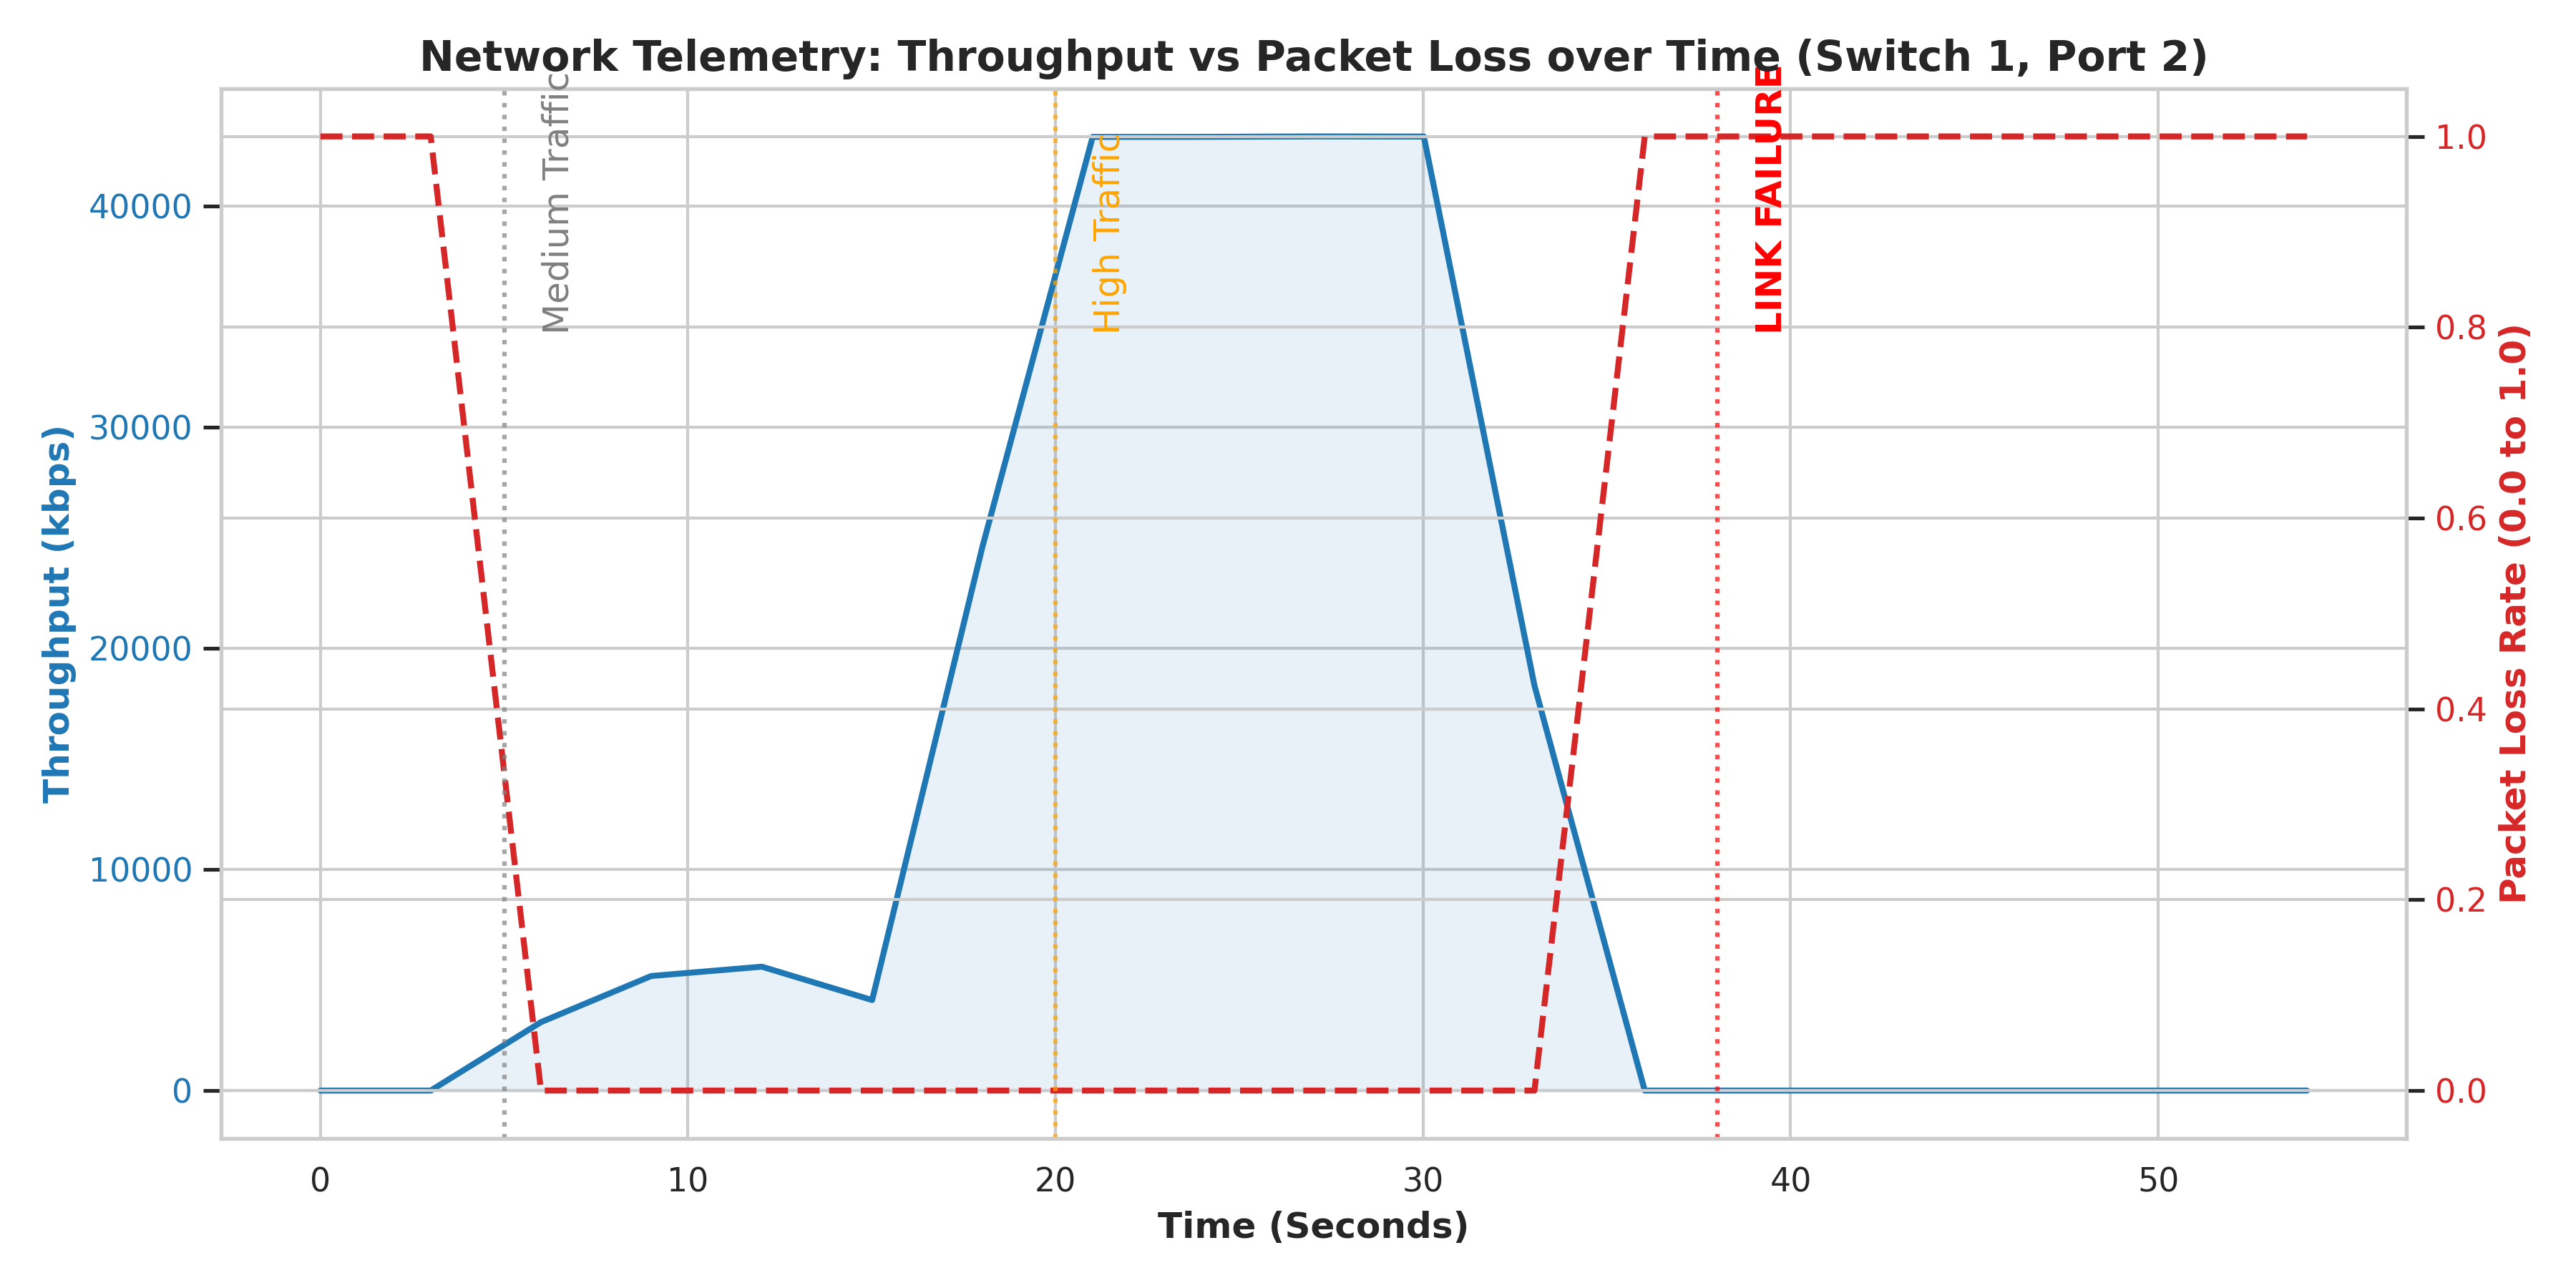
\includegraphics[width=0.9\textwidth]{figures/Telemetry_Graph.png}
\caption{Network telemetry over time (switch~1, port~2): throughput versus packet-loss rate.
Loss saturates when the monitored link fails, the transition the detector must catch.}
\label{fig:telemetry}
\end{figure}

\subsection{Autonomous Decision Testing}
On the illustrative live test the trained agent behaved deterministically: it took no action
on minor latency increases and initiated recovery only on genuine link failures.
\begin{verbatim}
Network State: NORMAL TRAFFIC     [tput 1500.0, loss 0.00, delay 1.5] -> Do Nothing
Network State: MEDIUM CONGESTION  [tput 4500.0, loss 0.02, delay 5.0] -> Do Nothing
Network State: SEVERE FAULT       [tput 0.0,    loss 1.00, delay 15.0]-> Reroute (Recovery)
\end{verbatim}

\subsection{Fault-Detection Accuracy}
Moving from the illustrative test to a rigorous evaluation, the detector was trained and
tested on leakage-free stratified splits (oversampling applied to the training split only),
averaged over five seeds. It reaches the metrics in Table~\ref{tab:detect} and never raises a
false alarm on the held-out normal class. % [VERIFIED evaluate_agent.py]
On identical splits, two lightweight classifiers match or beat the PPO agent
(Table~\ref{tab:baselines}): $k$-NN reaches $1.000$ F1 and logistic regression $0.975$,
against $0.962$ for PPO. % [VERIFIED compare_methods.py]
Detection quality therefore does not depend on the learning algorithm, which is why the
final design keeps detection simple and reserves learning for the recovery policy.

\begin{table}[t]
\centering
\caption{Held-out fault detection (5 seeds, mean $\pm$ std). % [VERIFIED evaluate_agent.py]}
\label{tab:detect}
\begin{tabular}{lc}
\toprule
Metric & Value \\
\midrule
Accuracy & $0.940 \pm 0.012$ \\
Precision & $1.000 \pm 0.000$ \\
Recall & $0.927 \pm 0.015$ \\
F1 & $0.962 \pm 0.008$ \\
\bottomrule
\end{tabular}
\end{table}

\begin{table}[t]
\centering
\caption{Method comparison, held-out F1 (5 seeds). % [VERIFIED compare_methods.py]}
\label{tab:baselines}
\begin{tabular}{lcccc}
\toprule
Method & Acc. & Prec. & Rec. & F1 \\
\midrule
Loss-threshold rule & 0.695 & 1.000 & 0.630 & 0.773 \\
Logistic regression & 0.960 & 1.000 & 0.952 & 0.975 \\
$k$-NN ($k{=}5$) & 1.000 & 1.000 & 1.000 & \textbf{1.000} \\
PPO agent & 0.940 & 1.000 & 0.927 & 0.962 \\
\bottomrule
\end{tabular}
\end{table}

\subsection{Fault Localisation at Scale}
A per-port telemetry classifier could not localise faults (measured precision
$\approx 0.10$), so the framework uses OpenFlow port-status. On the full fault set it
localises every injected hard fault across both topologies with no congestion false alarms
(Table~\ref{tab:localize}), generalising to the unseen second topology by construction.
% [VERIFIED docs/p1_detection_results.txt]

\begin{table}[t]
\centering
\caption{Hybrid fault localisation. Mean latency $0.21$~s; the production controller is
event-driven. % [VERIFIED docs/p1_detection_results.txt]}
\label{tab:localize}
\begin{tabular}{lcccc}
\toprule
Topology & Hard faults & Localised & Accuracy & Congestion FA \\
\midrule
mesh & 10 & 10 & $1.000$ & 0 \\
mesh2 & 9 & 9 & $1.000$ & 0 \\
\midrule
\textbf{Overall} & \textbf{19} & \textbf{19} & $\mathbf{1.000}$ & \textbf{0} \\
\bottomrule
\end{tabular}
\end{table}

\subsection{Autonomous Recovery (\texttt{OFPFlowMod})}
The controller installs backup \texttt{OFPFlowMod} rules and restores connectivity with no
sustained loss. Two variants are measured (Table~\ref{tab:variants}): an event-driven
controller that triggers on the OpenFlow port-status event recovers within $40\pm13$~ms,
while a controller driven by the periodic telemetry decision is bounded by the three-second
poll at $3.4\pm0.6$~s. % [VERIFIED docs/recovery_latency_results.txt]
Actuation itself is immediate in both cases. Data-plane round-trip time is $31.1$~ms
($3.5$~ms jitter) on the two-hop primary and $18.1$~ms ($1.4$~ms jitter) on the one-hop
backup. Against an OpenFlow fast-failover baseline (Table~\ref{tab:offail}), both mechanisms
recover a locally observable node fault at comparable speed, but per-switch fast-failover
cannot recover a single mid-link fault that the near switch never observes, whereas the
global-view controller reroutes both endpoints in about $40$~ms.
% [VERIFIED failover_agent.py, measure_recovery.py]

\begin{table}[t]
\centering
\caption{Recovery time by controller variant (single mid-link fault).
% [VERIFIED docs/recovery_latency_results.txt]}
\label{tab:variants}
\begin{tabular}{lcc}
\toprule
Variant & Recovery time & Bounded by \\
\midrule
Event-driven (port-status) & $40\pm13$~ms & OF event $\rightarrow$ flow mod \\
PPO-driven (telemetry) & $3.4\pm0.6$~s & 3~s statistics poll \\
\bottomrule
\end{tabular}
\end{table}

\begin{table}[t]
\centering
\caption{Recovery by mechanism and fault type. % [VERIFIED failover_agent.py]}
\label{tab:offail}
\begin{tabular}{lcc}
\toprule
Mechanism & Node fault & Single mid-link fault \\
\midrule
Fast-failover (\texttt{OFPGT\_FF}) & $52\pm10$~ms & \textbf{no recovery} \\
Controller reroute (ours) & $40\pm13$~ms & $40\pm13$~ms \\
\bottomrule
\end{tabular}
\end{table}

\subsection{Best-Path Resolution}
After the primary path fails, the live QoS of each survivor is measured and each strategy is
mapped to its chosen path. Composite QoS is $\text{tput}-0.05\,\text{lat}-0.2\,\text{loss}$
(Table~\ref{tab:resolve}). The resolver beats the loss-blind baselines (fixed-failover and
shortest-path) in three of five scenarios, is never worse than a strong load-aware
widest-path router, and clearly beats it when loss sits on the high-capacity path
(\texttt{loss\_C\_fat}: $6.1\pm3.6$ against $-13.2\pm4.5$ over eight seeds). It matches a
ground-truth oracle in every scenario; because the loss gaps ($16$--$33$ points) sit well
outside the $\sigma=0.05$ observation noise, matching the oracle here is a robustness check
rather than an optimality claim. % [VERIFIED docs/s2_5_results.txt]

\begin{table}[t]
\centering
\footnotesize
\caption{Composite QoS by strategy, 5 scenarios $\times$ 8 seeds (mean).
% [VERIFIED docs/s2_5_results.txt]}
\label{tab:resolve}
\begin{tabular}{lrrrrrr}
\toprule
Scenario & fixed & short & widest & rand & \textbf{resolver} & oracle \\
\midrule
congest\_B & $-0.1$ & $-0.1$ & $12.7$ & $4.3$ & $\mathbf{12.7}$ & $12.7$ \\
loss\_B & $-4.8$ & $-4.8$ & $8.4$ & $0.2$ & $\mathbf{8.4}$ & $8.4$ \\
congest\_loss\_B & $-5.2$ & $-5.2$ & $9.6$ & $0.6$ & $\mathbf{9.6}$ & $9.6$ \\
congest\_C\_ctrl & $5.4$ & $5.4$ & $5.4$ & $-0.4$ & $\mathbf{5.4}$ & $5.4$ \\
loss\_C\_fat & $6.1$ & $6.1$ & $-13.2$ & $-2.4$ & $\mathbf{6.1}$ & $6.1$ \\
\bottomrule
\end{tabular}
\end{table}

\subsection{Online Learning (Day by Day)}
On a nine-day non-stationary schedule, the degradation drifts between survivors and the
decisive signal (loss) is not observable at decision time, so the best path must be learned
from realised rewards. Three agents share the day-zero policy: an online reinforcement
learner, a frozen model, and an adaptive sliding-window bandit. As the world drifts, the
frozen model collapses from $13.0$ to $-11.0$, while the online learner and the adaptive
baseline relearn the best path (Table~\ref{tab:learn}, Figure~\ref{fig:learncurve}). Over
eight seeds and an exact paired sign-flip permutation test, the online learner exceeds the
frozen model in the late regime with $p=0.0039$, shows no net forgetting, and matches the
adaptive baseline ($4.0$ versus $3.8$; $p=0.547$). % [VERIFIED docs/s3_4_results.txt]

\begin{table}[t]
\centering
\footnotesize
\caption{Mean recovery reward per day over 8 seeds
($r=\text{tput}-0.5\,\text{loss}-t_{\text{rec}}$). % [VERIFIED docs/s3_4_results.txt]}
\label{tab:learn}
\begin{tabular}{crrrc}
\toprule
Day & online & frozen & adaptive & $p(\text{degrade B})$ \\
\midrule
0 & $10.2$ & $13.0$ & $8.4$ & $0.90$ \\
2 & $8.7$ & $11.3$ & $9.1$ & $0.70$ \\
4 & $-1.6$ & $-1.7$ & $-1.7$ & $0.50$ \\
6 & $1.3$ & $0.3$ & $-0.5$ & $0.30$ \\
7 & $3.1$ & $-9.1$ & $1.0$ & $0.20$ \\
8 & $4.8$ & $-11.0$ & $6.7$ & $0.10$ \\
\bottomrule
\end{tabular}
\end{table}

\begin{figure}[t]
\centering
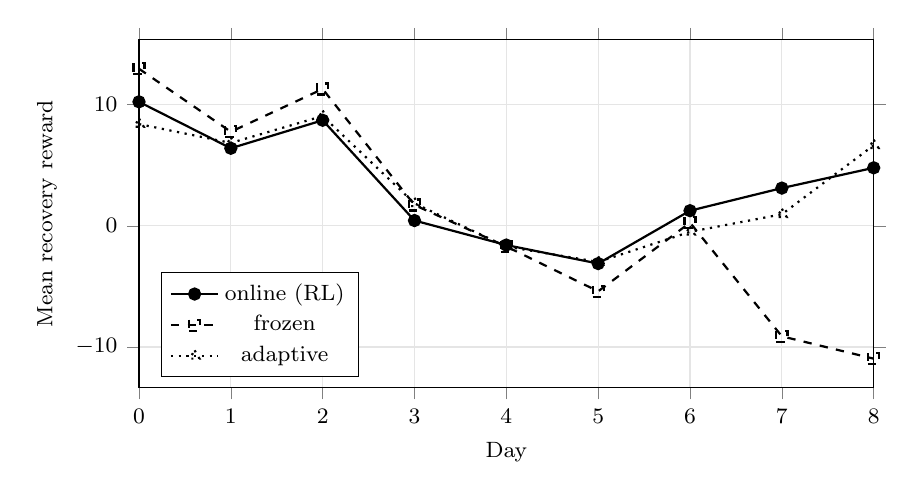
\begin{tikzpicture}
\begin{axis}[width=0.9\textwidth, height=6cm, font=\footnotesize,
  xlabel={Day}, ylabel={Mean recovery reward}, xmin=0, xmax=8,
  xtick={0,1,2,3,4,5,6,7,8}, legend pos=south west, grid=both,
  grid style={gray!20}, tick align=outside]
\addplot[thick,mark=*] coordinates
  {(0,10.238)(1,6.404)(2,8.716)(3,0.437)(4,-1.586)(5,-3.115)(6,1.250)(7,3.116)(8,4.790)};
\addlegendentry{online (RL)}
\addplot[thick,dashed,mark=square] coordinates
  {(0,12.968)(1,7.764)(2,11.298)(3,1.717)(4,-1.708)(5,-5.407)(6,0.263)(7,-9.120)(8,-10.966)};
\addlegendentry{frozen}
\addplot[thick,dotted,mark=triangle] coordinates
  {(0,8.401)(1,6.844)(2,9.063)(3,1.855)(4,-1.711)(5,-2.980)(6,-0.496)(7,0.953)(8,6.651)};
\addlegendentry{adaptive}
\end{axis}
\end{tikzpicture}
\caption{Mean recovery reward per day over eight seeds. The frozen policy collapses as the
world drifts, while the reinforcement-learning (online) policy and the adaptive bandit both
relearn the best path and recover. % [VERIFIED docs/s3_4_results.txt]}
\label{fig:learncurve}
\end{figure}

\subsection{Live Integration Success (End-to-End)}
Finally, all stages run in a single live process over a drifting five-day schedule with
twenty faults (Table~\ref{tab:e2e}). The controller detects every fault from port-status in
about $0.25$~s, installs a valid recovery path on all twenty, and achieves full connectivity
whenever it chooses a currently healthy survivor. The single reachability blip is a case
where, before adapting, the controller chose the survivor that was about to become lossy
under load; a valid path was still installed, so this is a learning signal, not a recovery
failure. Over the run the learner shifts its path preference from~C to~B as the world drifts.
% [VERIFIED docs/s4_1_results.txt]

\begin{table}[t]
\centering
\footnotesize
\caption{End-to-end run: one live process, 5 drifting days, 20 faults. Day-mean reward
$[18.7, 17.4, 10.1, -22.9, 10.7]$. % [VERIFIED docs/s4_1_results.txt]}
\label{tab:e2e}
\begin{tabular}{lc}
\toprule
Outcome & Result \\
\midrule
Faults detected (port-status, $\sim$0.25~s) & $20/20$ \\
Valid recovery path installed & $20/20$ \\
Full reachability on a healthy-survivor choice & $15/15$ \\
Reachability overall & $19/20$ \\
Accepted learner updates & 3 \\
Resolver preference (day 0 $\rightarrow$ final) & C $\rightarrow$ B \\
\bottomrule
\end{tabular}
\end{table}

\section{Summary}
The environment was configured with Mininet and Ryu, and the key engineering challenges (the
zero-packet anomaly and dataset class imbalance) were resolved. Beyond the initial detection
testbed, the framework experiments confirmed accurate localisation ($19/19$), fast
event-driven recovery ($\sim$40~ms) that beats fast-failover on mid-link faults, loss-aware
path selection that beats loss-blind recovery and matches an oracle, and an online learner
that adapts day by day while a frozen model collapses. A single end-to-end run demonstrated
all stages operating together on one live topology.

% =====================================================================
\chapter{Standards and Design Constraints}
This chapter describes the standards the project complies with and the design constraints
considered, followed by a cost analysis and the project timeline.

\section{Compliance with the Standards}
\subsection{Software Standards}
The implementation follows widely accepted software standards. The control-plane and
evaluation code is written in Python following the PEP~8 style guide, uses version control
(Git) for reproducibility, and depends only on permissively licensed open-source software
(Mininet, Open vSwitch, Ryu, and standard Python libraries), which avoids licensing
conflicts. The controller is built on the Ryu framework and adheres to its application model,
and results are made reproducible through pinned dependency versions and documented run
commands. Data files use standard, portable formats (CSV and JSON).

\subsection{Hardware Standards}
The project runs on commodity x86-64 hardware and does not require specialised or proprietary
equipment. A standard multi-core laptop or desktop with at least 16~GB of RAM is sufficient,
since the network is emulated in software. Because no custom hardware is involved, the work
conforms to ordinary consumer-hardware safety and interoperability expectations, and it can
be reproduced on any machine capable of running an Ubuntu Linux virtual machine.

\subsection{Communication Standards}
All network communication follows established open standards. The data plane uses the
OpenFlow~1.3 protocol between the controller and Open vSwitch, switch configuration uses the
OVSDB management protocol, and host traffic uses standard TCP/IP (with ICMP and UDP for
reachability and load generation). Adherence to these standards means the design is not tied
to a single vendor and can, in principle, be ported to any OpenFlow-compliant data plane.

\section{Design Constraints}
\subsection{Economic Constraint}
The project was built entirely on free, open-source software and commodity hardware the team
already owned, so the direct cost is negligible (see the cost analysis in
Section~\ref{sec:cost}). This makes the approach affordable for academic and small-operator
settings, but it also means the evaluation is limited to what commodity emulation can
represent rather than carrier-grade hardware.

\subsection{Environmental Constraint}
Because the system is evaluated in software emulation on a single machine, its direct
environmental footprint is small (the electricity used by one laptop or virtual machine). At
deployment scale, a self-healing controller can indirectly reduce environmental impact by
recovering faults automatically, avoiding unnecessary truck rolls and manual intervention,
and by keeping utilisation efficient.

\subsection{Ethical Constraint}
The project raises few ethical concerns because it operates on network-level telemetry
(throughput, loss, delay, and port state) and does not inspect packet payloads or personal
data. The evaluation reports results honestly, including negative findings (for example that
a simple classifier matches the learned detector), and the released artifact allows
independent verification, consistent with good research ethics.

\subsection{Health and Safety Constraint}
The work involves only software running on standard computers and poses no physical health or
safety risk to users or operators. In a production setting, the actuation logic installs
flow rules fail-secure and validates learning updates before accepting them, which reduces
the risk of an automated action degrading a live network.

\subsection{Social Constraint}
Reliable networks are increasingly critical to education, healthcare, commerce, and emergency
services. By reducing downtime and manual intervention, an autonomous self-healing controller
can improve service continuity for the communities that depend on these networks, especially
where skilled network operators are scarce.

\subsection{Political Constraint}
The project uses vendor-neutral open standards (OpenFlow, OVSDB, TCP/IP) and open-source
tools, so it does not depend on any single vendor or jurisdiction. This neutrality supports
adoption across organisations and regions and avoids the policy risks associated with
proprietary, closed platforms.

\subsection{Sustainability}
The design is sustainable both technically and economically. It relies on maintained
open-source platforms, runs on hardware that can be reused for future SDN and AI research,
and is documented and version-controlled so that it can be extended rather than rebuilt.
The lightweight, emulation-based methodology keeps power consumption and cost low while
providing a foundation for larger studies.

\section{Cost Analysis}
\label{sec:cost}
This section gives a financial overview for implementing the self-healing SDN system with
Mininet and the Ryu controller. All experiments run on personal laptops using open-source
tools, keeping cost low while maintaining sustainability. Table~\ref{tab:cost} summarises the
estimated cost.

\begin{table}[t]
\centering
\footnotesize
\caption{Project cost summary.}
\label{tab:cost}
\begin{tabular}{p{3.2cm}p{3.6cm}p{2.2cm}p{4.4cm}}
\toprule
Category & Item & Cost (USD) & Notes \\
\midrule
Operating system & Ubuntu Linux & \$0 & Open-source, compatible with Mininet \\
SDN controller & Ryu / ODL / ONOS & \$0 & Free, open-source controllers \\
Learning frameworks & Stable-Baselines3, etc. & \$0 & Permissive open-source licences \\
Network emulator & Mininet & \$0 & Free, open-source \\
Monitoring tools & Wireshark, iperf & \$0 & Open-source \\
Workstation (per developer) & Laptop, multi-core, 16~GB RAM & \$700--\$1500 & Existing or
minimal upgrade; GPU optional \\
External storage & 1~TB HDD/SSD & \$40--\$60 & Datasets, logs, checkpoints \\
Connectivity & Broadband & \$10--\$20/mo & Updates, repository access \\
Documentation & Printing, binding & \$10--\$15 & One-time submission cost \\
Miscellaneous & Electricity, stationery & \$15--\$25 & Minor recurring costs \\
\bottomrule
\end{tabular}
\end{table}

\noindent\textbf{Total estimated budget.} Using existing laptops (preferred), the project
cost is approximately \$75--\$100 in operational and documentation expenses; including a
laptop upgrade, it is \$750--\$1500. \textbf{Rationale and sustainability:} the work relies
entirely on open-source platforms (no licensing fees), reuses existing hardware, runs on
personal laptops to keep infrastructure cost low, and, because of the lightweight nature of
virtual simulation, keeps power consumption and environmental impact minimal.

\section{Gantt Chart}
For systematic management, the project is divided into stages, each tracked with a Gantt
chart.

\subsection{Gantt Chart 1: FYDP-1 (Planning \& Design Phase)}
This stage covers the literature review, requirement analysis, and system design.
\begin{figure}[h]
\centering
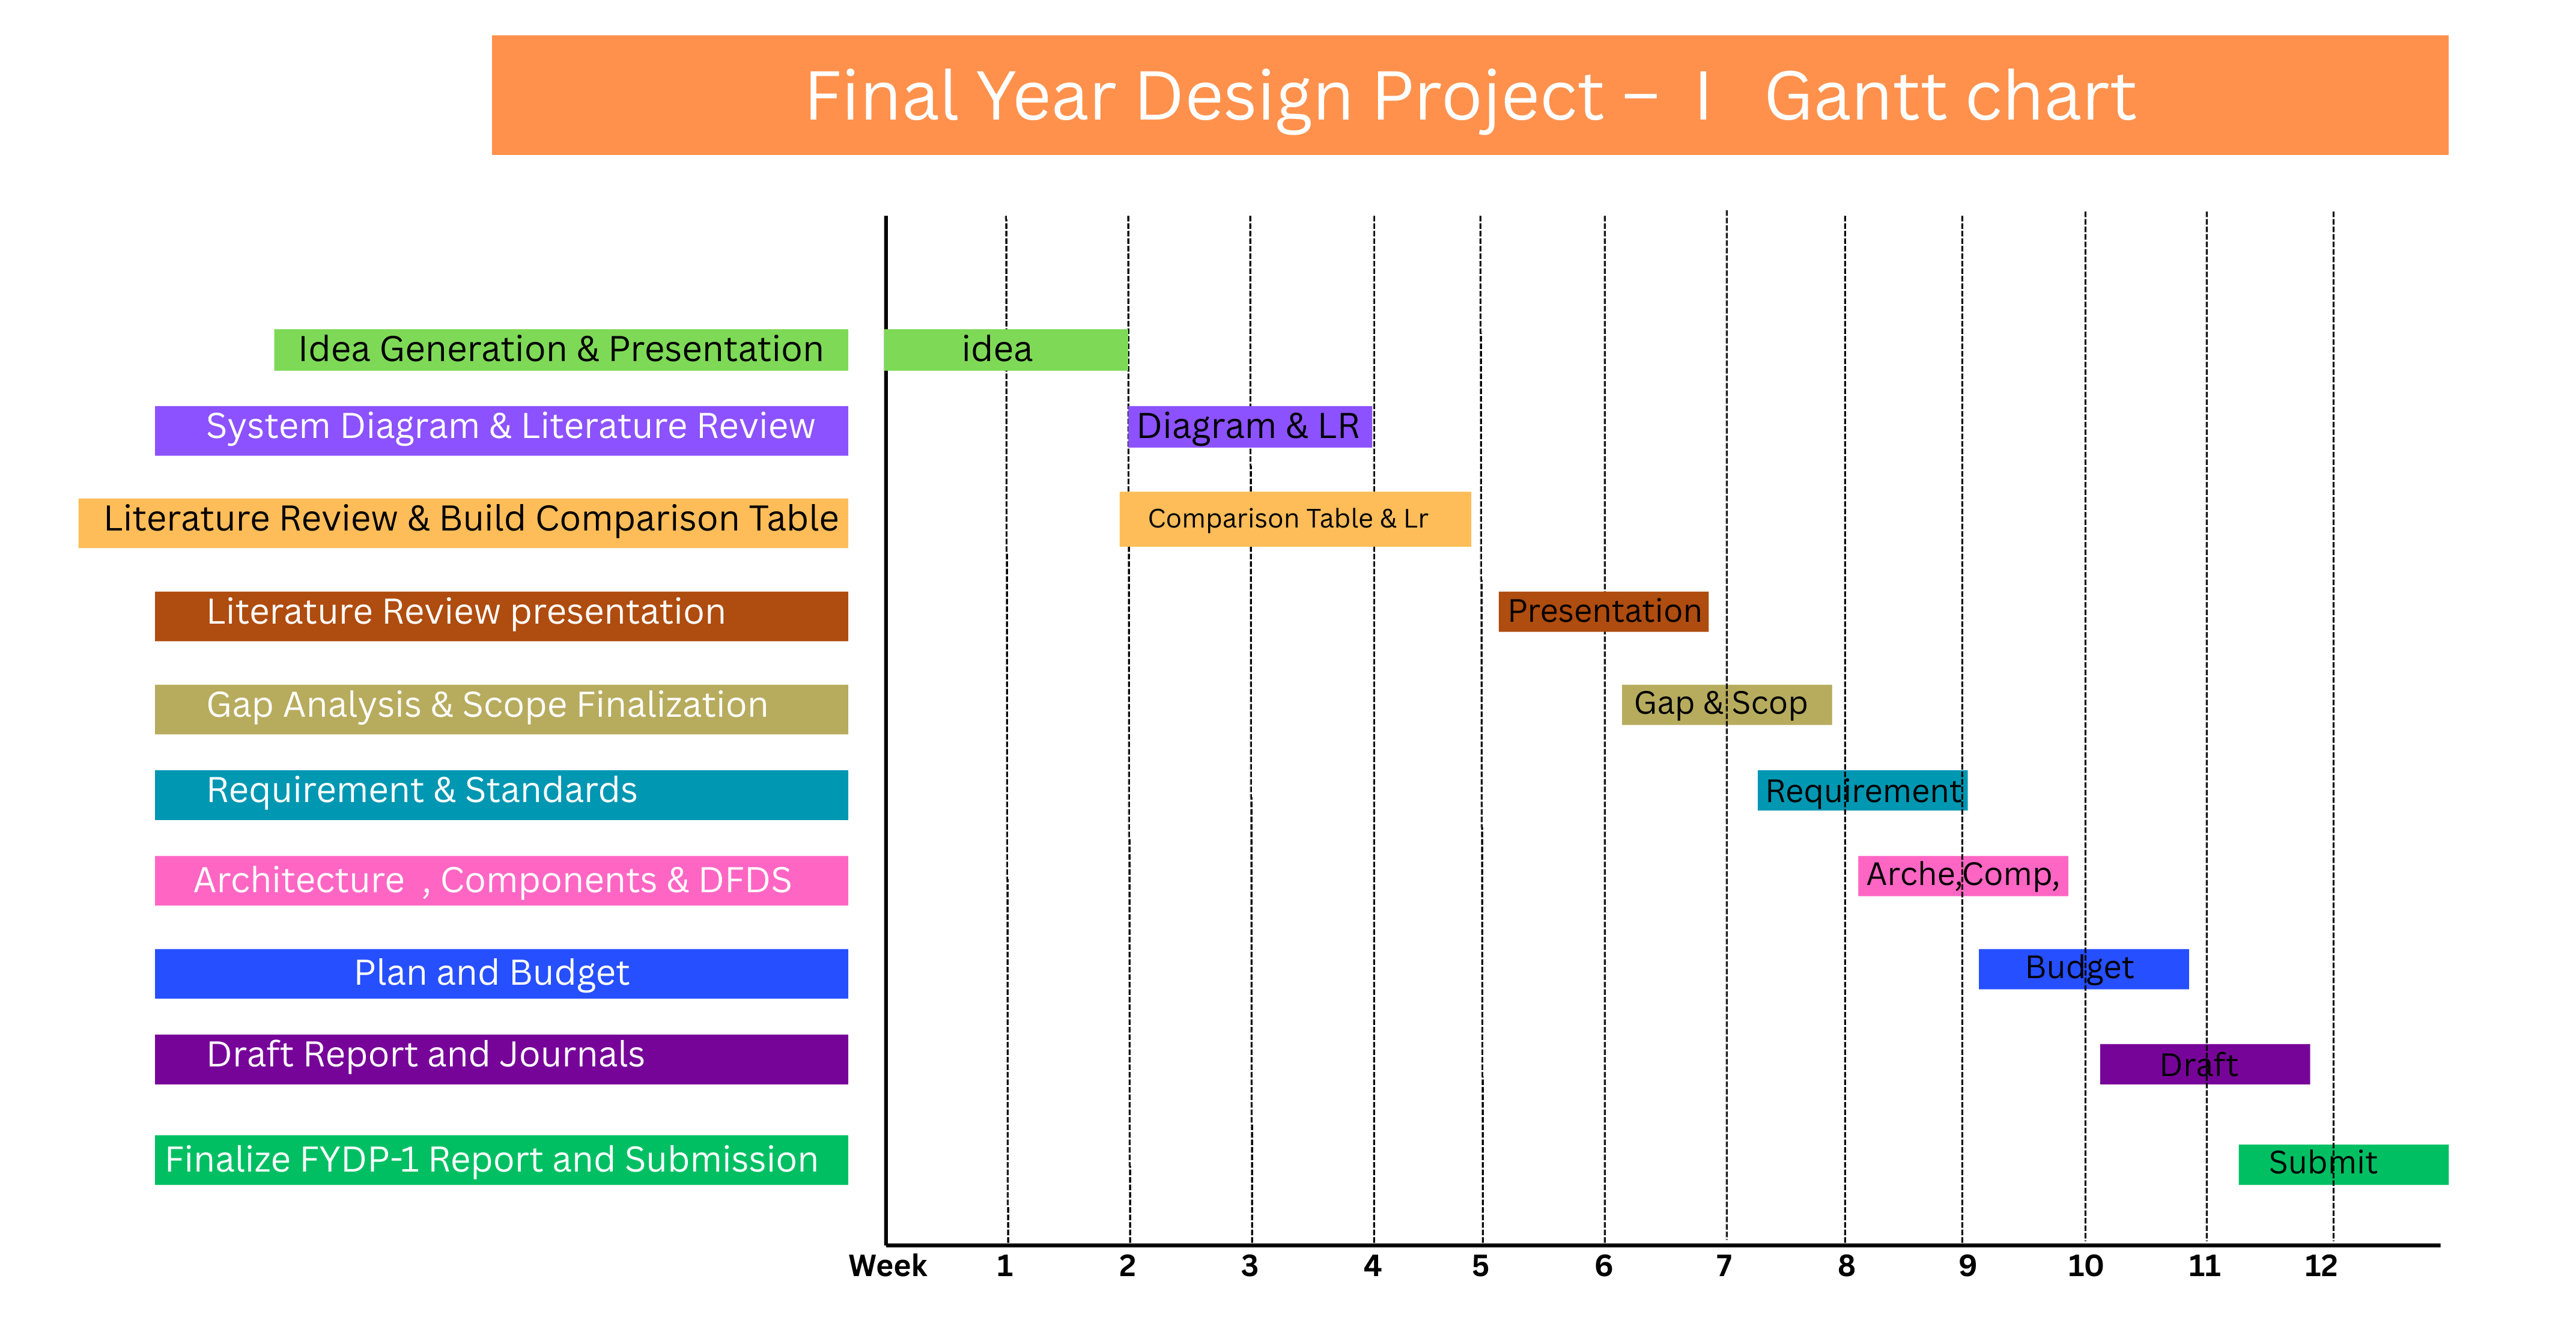
\includegraphics[width=\textwidth]{figures/gantt1.png}
\caption{Gantt Chart 1: FYDP-1 planning and design phase.}
\label{fig:gantt1}
\end{figure}

\subsection{Gantt Chart 2: FYDP-2 (Implementation Phase)}
In this phase the SDN environment is established and linked with the decision and learning
components.
\begin{figure}[h]
\centering
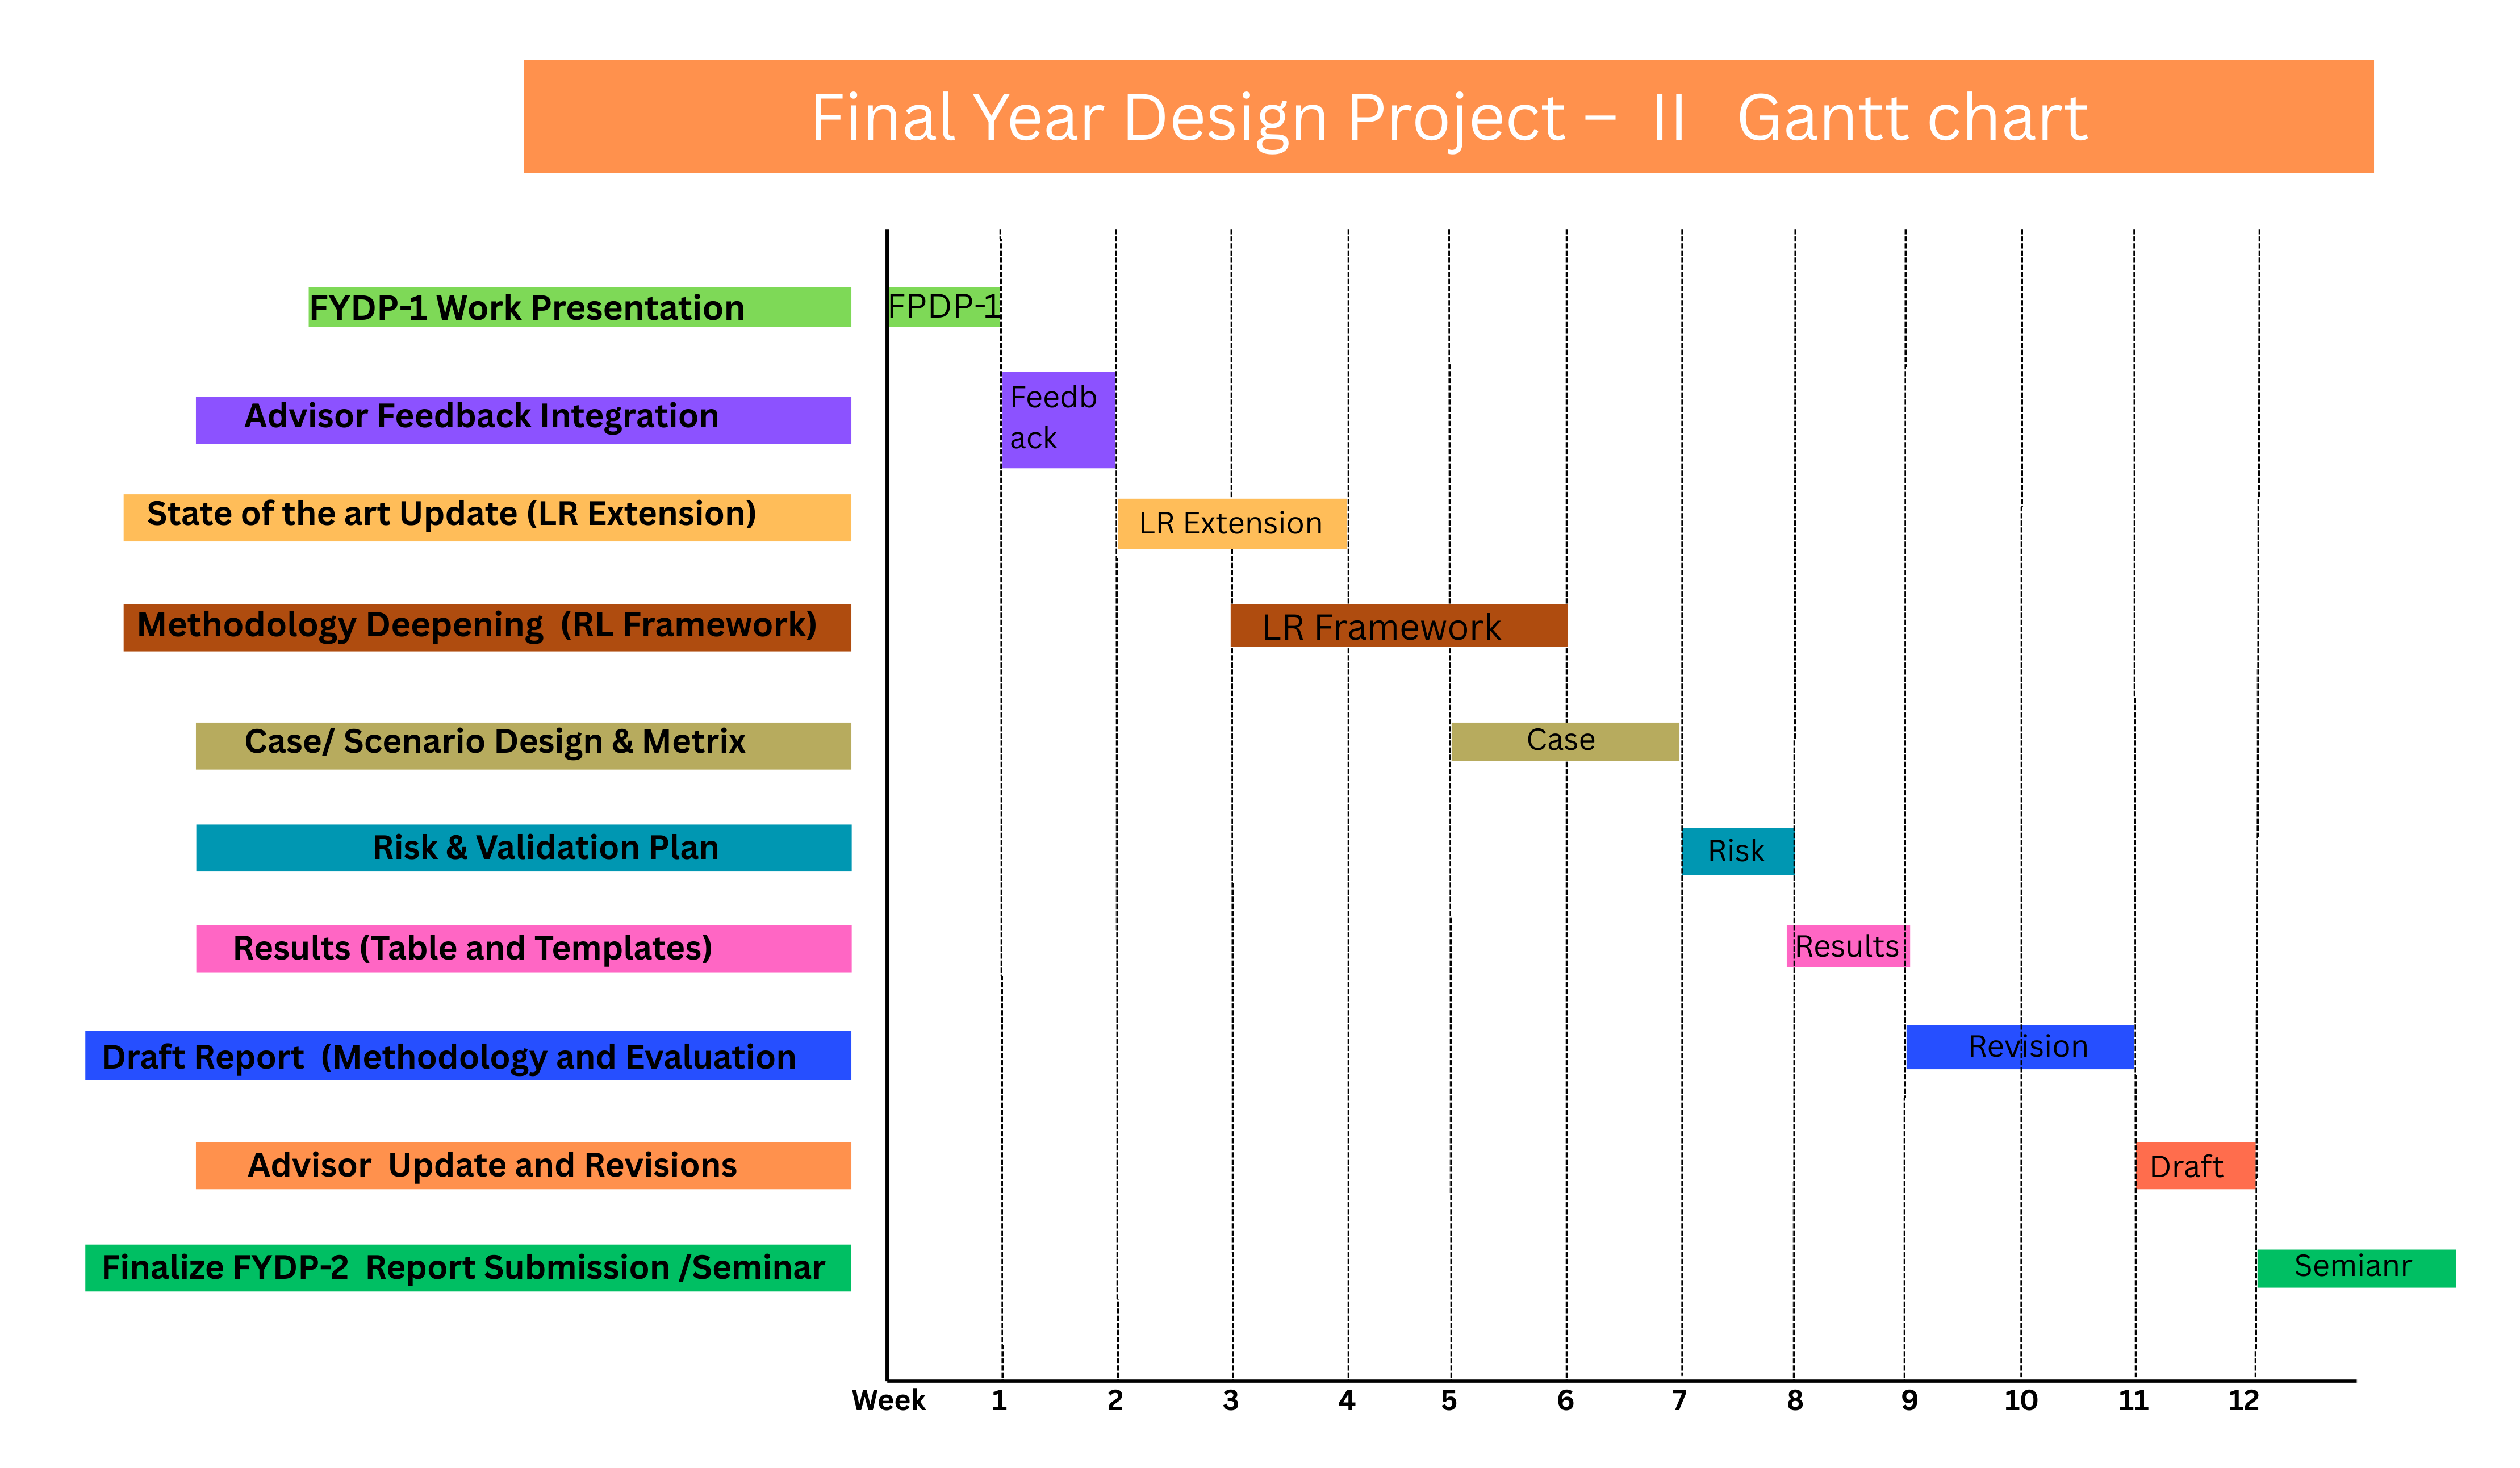
\includegraphics[width=\textwidth]{figures/gantt2.png}
\caption{Gantt Chart 2: FYDP-2 implementation phase.}
\label{fig:gantt2}
\end{figure}

\subsection{Gantt Chart 3: Testing and Evaluation Phase}
This stage focuses on testing the self-healing system, analysing performance results, and
preparing the final documentation.
\begin{figure}[h]
\centering
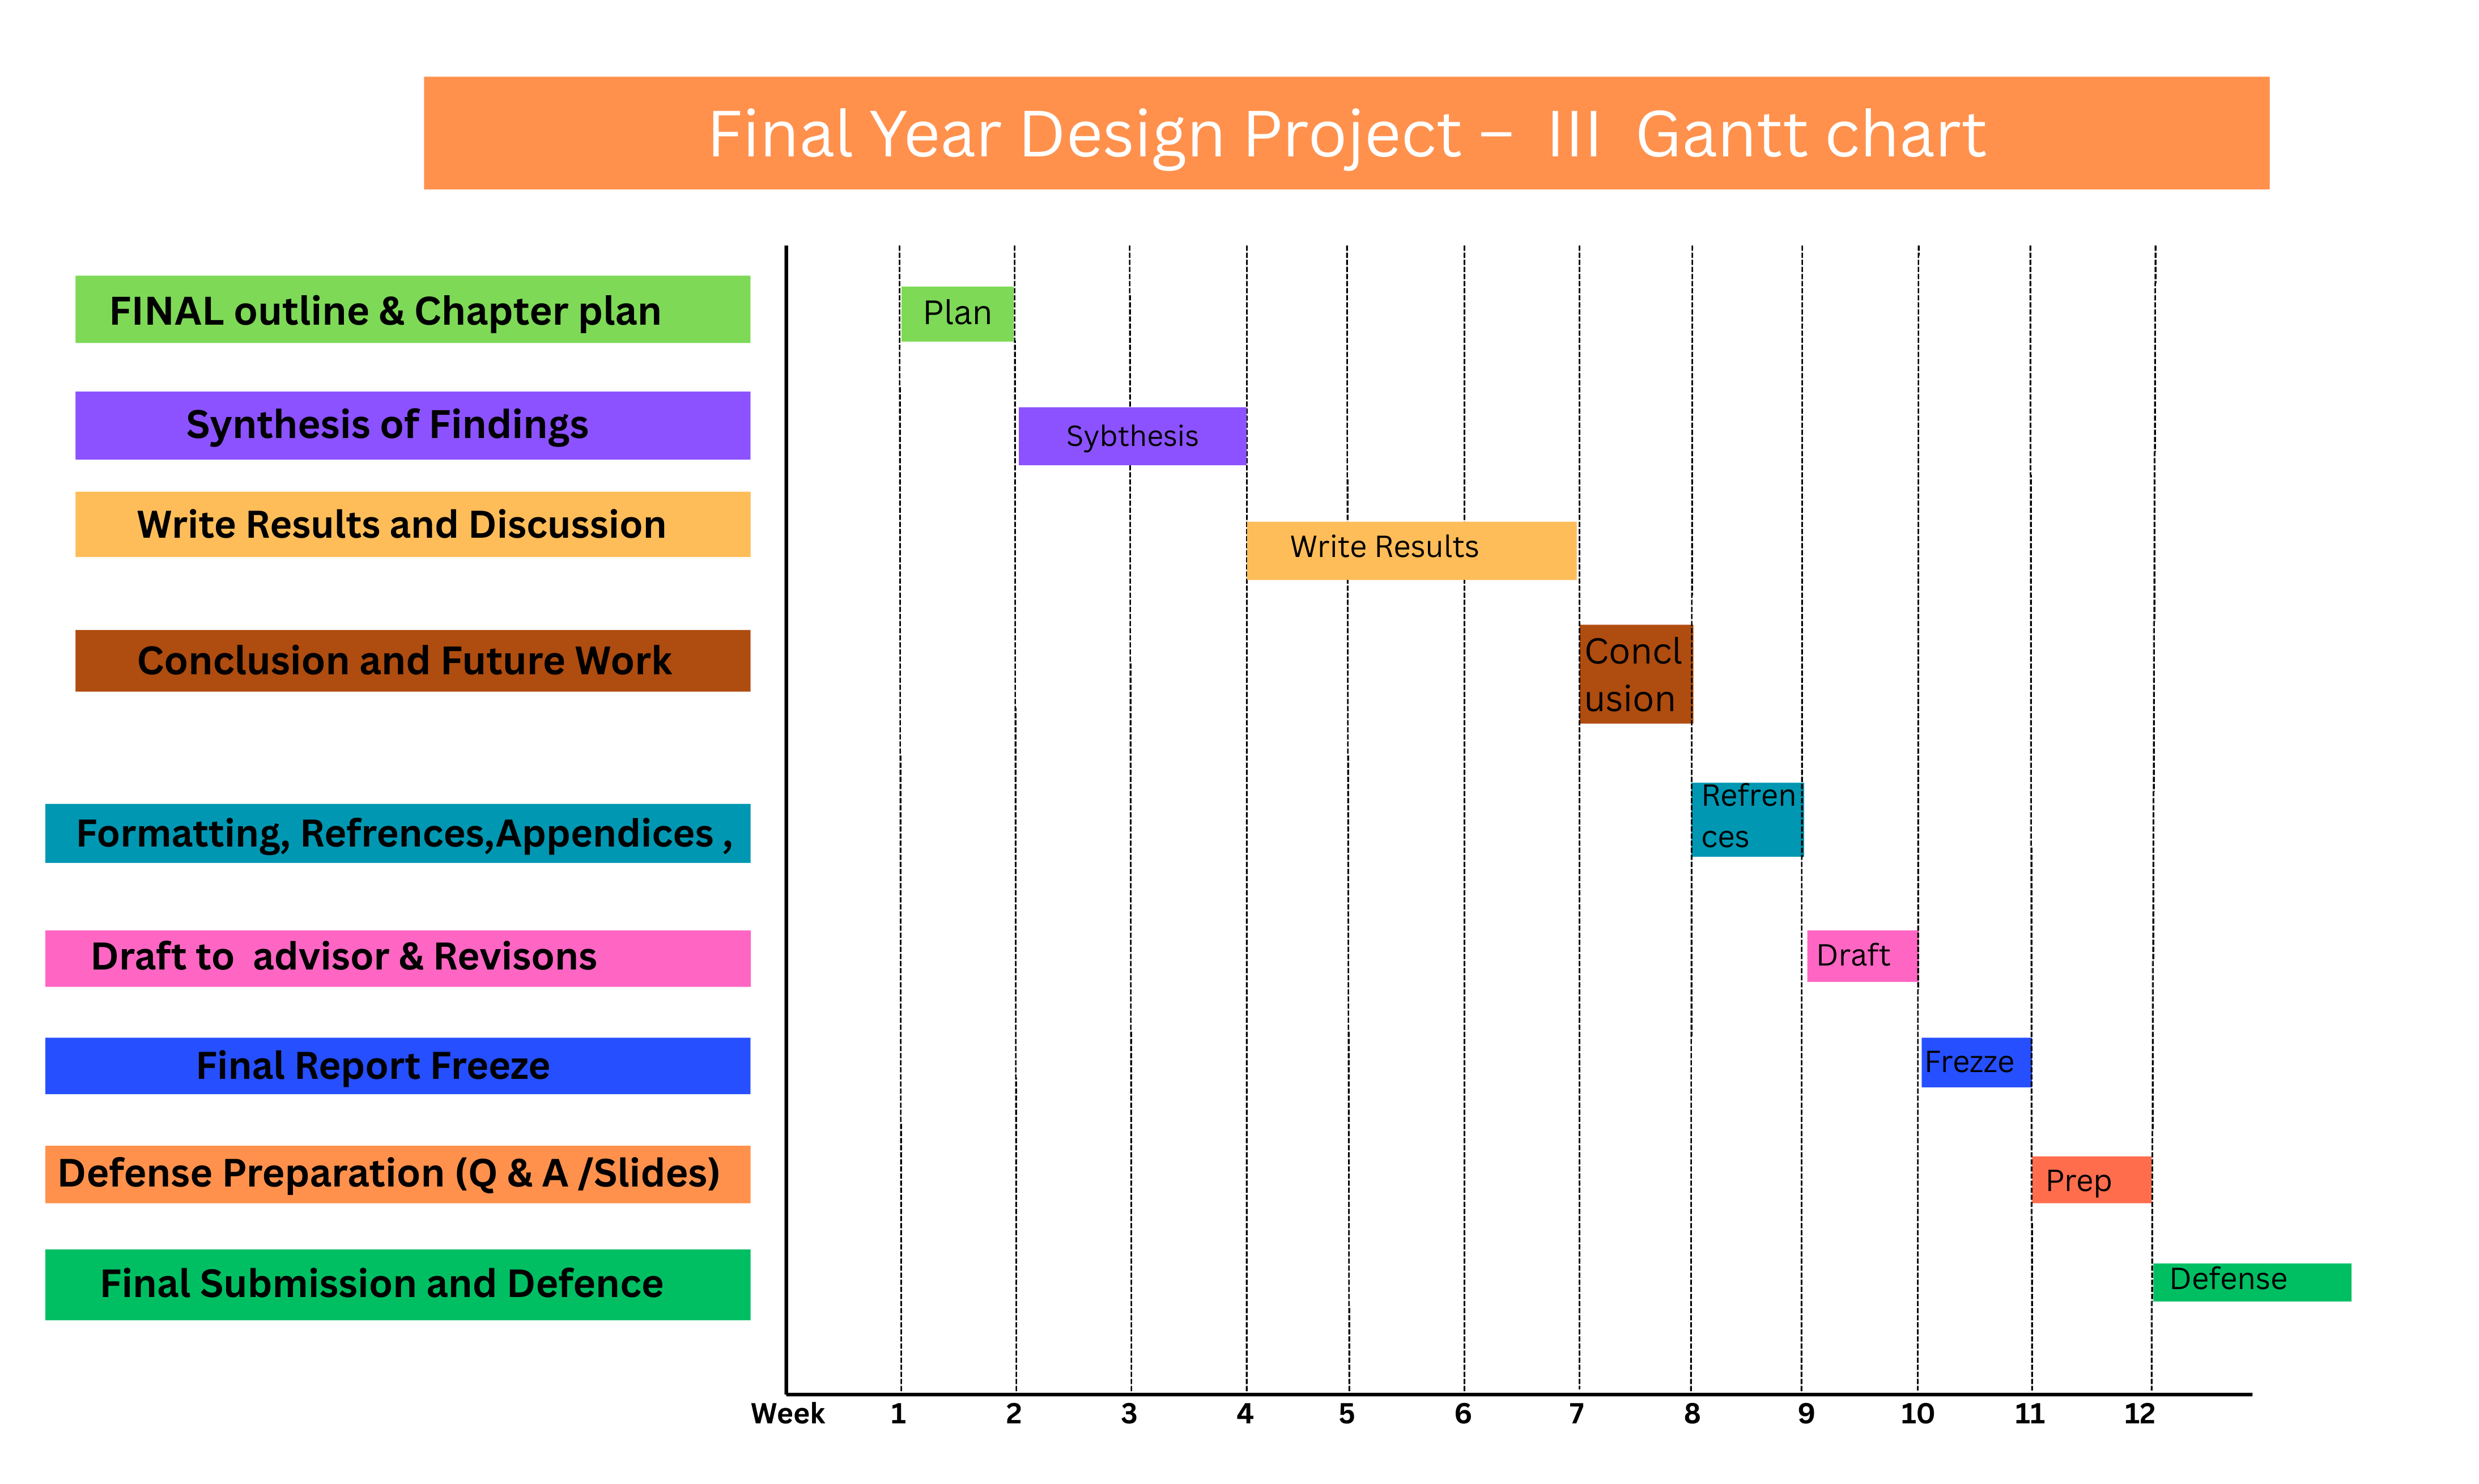
\includegraphics[width=\textwidth]{figures/gantt3.png}
\caption{Gantt Chart 3: testing and evaluation phase.}
\label{fig:gantt3}
\end{figure}

% =====================================================================
\chapter{Conclusion}
This phase of the Final Year Design Project has been completed successfully. Separating
network-state monitoring from the recovery decision through a modular design proved feasible,
and combining OpenFlow telemetry with a reinforcement-learning recovery policy allowed the
system to identify faults and recover autonomously. Crucially, the recovery decision is no
longer only a decision: the controller now translates it into \texttt{OFPFlowMod} messages
that update the switch flow tables and reroute traffic in real time, which was listed as
future work in the earlier phase and is now implemented. The evaluation extended from a small
detection testbed to a full framework, with accurate localisation, fast recovery, loss-aware
path selection, and day-by-day learning, each measured against honest baselines.

\section{Summary}
The system detects and localises faults, resolves the best surviving path, actuates recovery
with \texttt{OFPFlowMod}, and learns from the outcome to improve over time. Across the study
it localises every injected hard fault, restores connectivity within a bounded transient of
about $40$~ms, chooses paths at least as well as a strong load-aware baseline and better when
loss and bandwidth disagree, and keeps recovery quality high on a drifting network where a
frozen model collapses. A single end-to-end run demonstrated all stages operating together.
A consistent and honest finding is that the value lies in the integrated closed loop and in
placing learning where it matters (the sequential recovery policy), while a lightweight
classifier suffices for the stateless detection trigger.

\section{Limitation}
The evaluation uses emulation (Mininet and Ryu) at a scale sufficient for a controlled study,
so it does not capture the full complexity of a large production network. The resolution and
learning studies use two surviving paths after a single primary failure, and the learning
stage is a two-arm non-stationary problem with a binary decisive feature; extending to
topologies with three or more paths and richer feature interactions is future work. The
learning curve is trace-driven from live-measured QoS anchors, so a fully live multi-day loop
remains future work. Finally, the detection dataset is small and close to separable, which
inflates absolute detection scores; larger and less separable datasets would strengthen that
part of the evaluation.

% =====================================================================
\begin{thebibliography}{10}
\bibitem{boussaoud} K.~Boussaoud, A.~En-Nouaary, and M.~Ayache, ``Adaptive congestion
detection and traffic control in software-defined networks via data-driven multi-agent
reinforcement learning,'' \emph{Computers}, vol.~14, no.~6, p.~236, 2025.
\bibitem{huang} W.~Huang, W.~Gui, Y.~Li, Q.~Lv, J.~Zhang, and X.~He, ``Faulty links' fast
recovery method based on deep reinforcement learning,'' \emph{Algorithms}, vol.~18, no.~5,
p.~241, 2025.
\bibitem{kumar} N.~Kumar, E.~S. Groenewald, S.~Kulkarni, and K.~M. Ashifa, ``Self-healing
networks: AI-based approaches for fault detection and recovery,'' \emph{Power System
Technology}, vol.~47, no.~4, pp.~371--386, 2023.
\bibitem{neto} N.~V. de~Souza~Neto, D.~R.~C. Oliveira, M.~A. Gon\c{c}alves, F.~de~Oliveira
Silva, and P.~F. Rosa, ``A self-healing platform for the control and management planes
communication in softwarized and virtualized networks,'' in \emph{Proc. 10th Int. Conf. on
Cloud Computing and Services Science (CLOSER)}, 2020, pp.~415--422.
\bibitem{hammad} M.~Hammad, N.~Hewahi, and W.~Elmedany, ``Enhancing network intrusion recovery
in SDN with machine learning: An innovative approach,'' \emph{Arab Journal of Basic and
Applied Sciences}, vol.~30, no.~1, pp.~561--572, 2023.
\bibitem{jo} S.~Jo, J.~Y. Oh, Y.~T. Yoon, and Y.~G. Jin, ``Self-healing radial distribution
network reconfiguration based on deep reinforcement learning,'' \emph{Results in
Engineering}, vol.~22, p.~102026, 2024.
\bibitem{li} P.~Li \emph{et al.}, ``RLOps: Development life-cycle of reinforcement learning
aided open RAN,'' \emph{IEEE Access}, vol.~10, pp.~113808--113826, 2022.
\bibitem{younisse} L.~Zhou, J.~Li, H.~Wang, and Y.~Chen, ``Deep reinforcement learning-based
fault management for self-healing in 5G networks,'' \emph{IEEE Transactions on Network and
Service Management}, vol.~20, no.~2, pp.~189--202, 2023.
\bibitem{khan} M.~A. Khan, R.~Ahmad, and S.~R. Malik, ``AI-driven self-healing mechanisms in
software-defined networks: A comprehensive survey,'' \emph{Computer Networks}, vol.~237,
p.~110014, 2024.
\bibitem{sahu} A.~Sahu, V.~Venkatraman, and R.~Macwan, ``A reinforcement learning approach to
solve service restoration and load management simultaneously for distribution networks,''
\emph{IEEE Transactions on Smart Grid}, vol.~10, no.~5, pp.~4950--4960, 2019.
\end{thebibliography}

\end{document}
